\documentclass[letterpaper]{report}
\usepackage{xunicode,xltxtra,indentfirst,phonology,fontspec,paralist}
\usepackage{longtable,lscape,booktabs,graphicx,tabularx,url,multicol}
%\setromanfont[Mapping=tex-text]{Arial Unicode MS}
\setromanfont[Mapping=tex-text]{CharisSIL}
%\setromanfont[Mapping=tex-text]{Gentium}
%%% Vowel Chart
\usepackage{vowel}
\hyphenation{Lwi-ta-xo}

\newenvironment{wrdex}
{\begin{itemize}
  \setlength{\itemsep}{-1pt}
  \setlength{\parskip}{0pt}
  \setlength{\parsep}{0pt}}
{\end{itemize}}
\usepackage{covington}

\author{Ryan Smith}
\title{Lwitaxo}

\begin{document}
\maketitle
\tableofcontents

\chapter{Introduction}
This is a grammar made as a final project for the field methods of linguistics course and Indiana University.  The course consisted of original research conducted by students, and directed by Professor Robert Botne.  The research was conducted by working with a native speaker of the Lwitaxo language in class and in private interview sessions.

\section{Lwitaxo}
The language Lwitaxo , also spelled Lwitakho and Lwidakho, is a Bantu language from South East Kenya.  Its Guthrie Bantu zone classification is JE34.  Information from Ethnologue, \url{http://www.ethnologue.com/show_language.asp?code=ida}, is shown in table \ref{tab:ethnologue} on page \pageref{tab:ethnologue} and a map of where Lwitaxo is spoken is shown in figure \ref{fig:map}.

% Table generated by Excel2LaTeX from sheet 'Sheet1'
\begin{table}[p]
  \centering
  \caption{The Ethnologue entry for the Luidakho-Luisukha-Lutirichi languages.}
\begin{tabularx}{\textwidth}{lX}
    \addlinespace
    \toprule
    {\it Population } & 306,000 (1987 BTL), increasing. Idakho 65,000, Isukha 90,000, Tiriki 100,000 (Heine and Möhlig 1980). \\
    \midrule
    {\it Region } & Western Province, Kakamega District. \\
    {\it Language map } & Kenya, reference number 26 \\
    {\it Alternate names  } & Idakho-Isukha-Tiriki \\
    {\it Dialects } & Idakho (Idaxo, Itakho), Isukha (Isuxa, Lwisukha), Tiriki. High comprehension of Logooli [rag], but resistance to each other’s pronunciation. Lexical similarity: 70\% with Logooli, 52\% with Masaba [myx] (Uganda) and Luyia [luy]. \\
    \multicolumn{ 1}{l}{{\it Classification }} & Niger-Congo, Atlantic-Congo, Volta-Congo, Benue-Congo, Bantoid, Southern, Narrow Bantu, Central, J, Masaba-Luyia (J.30), Luyia \\
    \multicolumn{ 1}{l}{{\it }} & A member of macrolanguage Oluluyia [luy] (Kenya). \\
    {\it Language use } & GIDS 5. Home, community, religious services. All Ages. Positive attitude. \\
    {\it Language development } & Literacy rate in L1: Below 1\%. Literacy rate in L2: 15\%–25\%. Taught in primary schools. Bible portions: 2000. \\
    \bottomrule
    \end{tabularx}
  \label{tab:ethnologue}
\end{table}

\begin{figure}[p] \label{fig:map}
\caption{A map of languages in Kenya.  Lwitakho is number 26, in the enlarged section.}
\centering
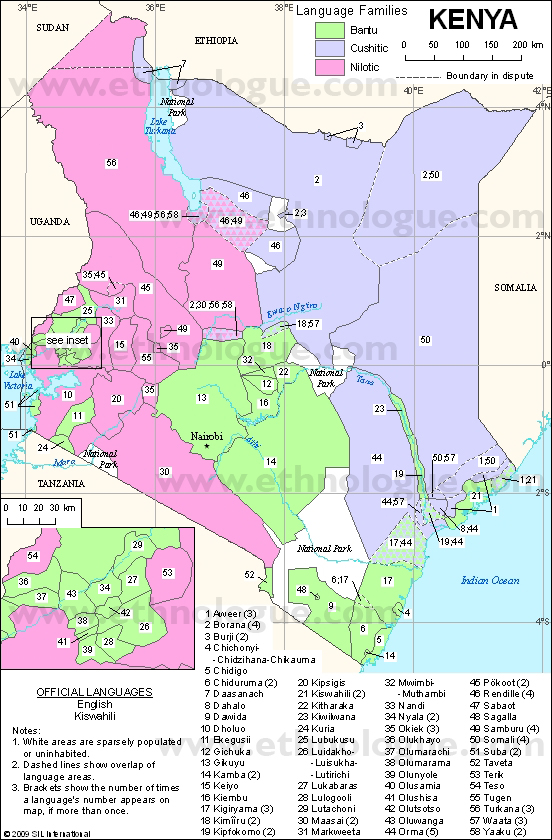
\includegraphics[width=.9\linewidth]{ken_eth}
\end{figure}

\section{Informant}
The informant for the elicitation sessions is a native speaker of Lwitaxo from Kenya.  She has lived in the United States for several years, attending graduate school, and also speaks the following languages: English, Swahili, Lubokusu, Lulokoli, Lukabarasi, and Kikuyu.

\chapter{Phonetics and Phonology}
\section{Sounds of Lwitaxo}
\subsection{Consonants}\label{sec:consonants}

\begin{minipage}{\linewidth}
\begin{tabular}{|l | c | c | c | c | c | c|}
\hline & Bilabial & Alveolar & P-alveo & Palatal & Velar & Glottal \\ \hline
Plosive & p (b)\footnote{Letters in parenthesis only exist as allophones} & t (d) & & & k (g) & \\\hline
Nasal & m & n & & \palnas{} & \engma{} & \\\hline
Affricates &  & ts (dz) & t\esh{} (d\ezh{}) & & & \\ \hline
Fricatives & \beta{} f & s & \esh{} & & x & h\\ \hline
Flap/Trill & &l \alvlatflap{}\footnote{it was discovered on the last day of research that l and \alvlatflap{} are possibly distinct phonemes, where as no difference was previously heard.  Due to this, the data in this grammar does not yet show this distinction.} r & & & & \\\hline
Glide & (w) & & & (j) & & \\ \hline
\end{tabular}
\end{minipage}

\subsection{Vowels}\label{sec:vowels}

Lwitaxo has a 5 vowel system.  There are high and mid front vowels, and high and mid back vowels.  The low vowel does not have a front/back distinction.

\begin{center}
\begin{vowel}[simple,three]
 \putcvowel{i}{1}
\putcvowel{\epsilon}{2}
\putcvowel{a}{5}
\putcvowel{\openo}{7}
\putcvowel{u}{8}
\end{vowel}
\end{center}

\begin{description}
\item[/i/] The high, unrounded, front vowel includes a large area of vowel space.  The actual realization of this sound when spoken includes everything from [i] to the upper limits of [e].  This means that the vowel written as `i' in this grammar might be pronounced as [i] in `tree', to [\openi] in `pit', to something that sounds a lot like [e] in `mate'.

\item[/\epsilon{}/] The mid, unrounded, front vowel is realized as [\epsilon{}], as in the English word `bed'.  The sound is transcribed with the letter `e' in this grammar.

\item[/u/]  The high, rounded, back vowel covers a very similar territory height-wise as /i/ does.  It is realized as [u] (as in English `moo') and also as [\openu{}] (as in English `lull').

\item[/\openo{}/] The mid, rounded back vowel is realized as [\openo] similar the English word `bog'.  In this grammar it is written as `o'.

\item[/a/] The /a/ is pronounced as a low back vowel.  It is the only low vowel in the vowel system.
\end{description}

\subsection{Tone}

Lwitaxo has two phonemic tones: high and low.  The low tone is the more neutral, and could also be referred to as `not-high.'  The tone is not fixed onto a syllable, but may move to a different syllable when a word is put in a sentence or a verb is conjugated

\begin{wrdex}
\item \emph{nimb\'a} `I sing' compared with \emph{nimba} `I sing.'
\item \emph{í\engma{}g\'u\beta{}u} `dress' compared with \emph{í\engma{}gu\beta{}u} `hippo'
\item \emph{ísímba} `lion compared with \emph{isimba} `hut for an unmarried man'
\item \emph{xulol\'a\engma{}ga} `I see you' but \emph{axulola\engma{}ga} `he/she sees you'
\item \emph{mb\'aja} `I play' but \emph{mbaja katí} `I play the game kati'
\end{wrdex}

\subsection{Length}

Vowel length is distinctive in Lwitaxo.  There appear to be 2 phonemic vowel lengths: long and short.  There do not seem to be many examples where the word differentiates only by vowel length, except for the the formation of the recent past perfective and the short form of the recent past imperfective.  In many cases where a vowel is deleted, there is a vowel lengthing as compensation.  Long vowels are notated with `:' following the vowel.

\begin{wrdex}
\item \emph{nd\ezh{}endi} `I walked (recent)' compared with \emph{nd\ezh{}e:ndi} `I was walking (recent)'
\item \emph{\engma{}wele} `I drank (recent)' compared with \emph{\engma{}we:le} `I was drinking (recent)'
\end{wrdex}

\section{Syllable Structure}
The possible syllable structure is (N)(C)(G)V.  The basic syllable is CV, and there are no codas allowed.  The only kinds of complex onsets allowed is for the consonant to be preceded by a nasal or succeeded by a glide. It is possible for the syllable to have both the nasal and the glide. The consonant without the onset, being only a vowel, seems to occur only in class 9 nouns\footnote{for a discussion of the noun class system see section \ref{sec:nounclasses}}, as well as 2nd and 3rd person singular verbs.

\fbox{(N)(C)(G)V}\\
% Table generated by Excel2LaTeX from sheet 'Sheet2'
\begin{tabular}{lll}
\addlinespace
\toprule
CV    & {\it \textbf{mi.hi.ka}} & `years' \\
V     & {\it \textbf{i}.tʃi.li.ʃi} & `bull' \\
NCV   & {\it tsi.\textbf{ndu}.ma} & `yams' \\
CGV   & {\it \textbf{xwi}.βi.li.la} & `to forget' \\
NCGV  & {\it i.si.\textbf{mbwa}} & `dog' \\
\bottomrule
\end{tabular}

\section{Phonological Rules}

\subsection{The nasals}

The nasals m,n,\palnas{}, and \engma{} appear to be distinctive sounds in Lwitaxo.

% Table generated by Excel2LaTeX from sheet 'Sheet2'
\begin{tabular}{ll}
\addlinespace
\toprule
{\it \textbf{mu}rio } & `thank you' \\
{\it  βwa\textbf{na} } & `childhood' \\
{\it  i\textbf{ɲi}ni\textbf{ɲi}ni } & `star' \\
{\it litʃu\textbf{ŋwa}} & `orange' \\
\bottomrule
\end{tabular}

Despite being distinctive, the nasals will assimilate to the place of articulation of a following consonant and neutralize the distinction of place of articulation in the nasal, as well as also causing the following consonant to voice.

  [nasal] \becomes [\alpha{} place] \inthe \environ [\alpha{} place]

  [+stop] \becomes [+voice] \inthe [+nasal] \environ

The sounds [h] and [\beta{}] also change when preceded by a nasal.  The \beta{} becomes a stop, [b], and the [h] acts like a [p]: voicing and becoming a stop [b] which causes the nasal to be realized as an [m].\\
\noindent\begin{minipage}{\linewidth}
\resizebox{\textwidth}{!}{ %
% Table generated by Excel2LaTeX from sheet 'Sheet2'
\noindent\begin{tabular}{llllll}
\addlinespace
\toprule
{\bf n + } & {\bf Results in} & {\bf Example} &       & {\bf Without n} &  \\
\midrule
{\bf n + p} & mb    & tsimbau & `woods'\footnote{as in different types of woods} & lupau & `wood' \\
{\bf n + t} & nd    & indana & `infant' & xatana &  `little infant' \\
{\bf n + k} & \engma{}g & ŋgulaŋga  & `I'm buying' & xukula & `to buy' \\
{\bf n + \beta{}} & mb    & mbimbitsa & `I'm boiling' & xu\beta{}imbitsa & `to boil' \\
{\bf n + h} & mb    & mbuja\engma{}ga & `I'm going home' & xuhuja & `to go home' \\
{\bf n + t\esh{}} & nd\ezh{} & ndʒenda\engma{}ga & `I'm walking' & xuts\esh{}enda & `to walk' \\
{\bf n + ts} & ndz   & indzu & `house' & xatsu & `little house' \\
{\bf n + j} & ndz   & indzuxa & `snake' & xajuxa & `little snake' \\
{\bf n + l} & nd & ndi & `I am' & ali & `he/she is' \\
{\bf n + l}\footnote{The reason for the two different results of `n+l' is unclear at this time: it may be a result of the two different l's: [l] and [\alvlatflap{}]} & n & nomaloma & `I speak' & ulomaloma & `you speak'\\
{\bf n + r} & nd & ndandula\engma{}ga & `I'm tearing' & xurandula & `to tear'\\
\bottomrule
\end{tabular}}
\normalsize
\end{minipage}

\subsection{Deletion of stop after a nasal}
When there are two syllables in a row which both have the nasal+consonant onset, then the consonant of the first of these syllables is deleted.

\fbox{NC...NC \becomes N...NC}

Example: \emph{i\engma{}gombe} is pronounced [i\engma{}ombe], however the diminutive form of cow, \emph{xakombe}, shows an underlying k (expected to turn into a g after the nasal of the class 9 prefix, see section \ref{sec:nounclasses}) which is not present in the pronunciation of the word.  The same situation occurs with [\engma{}] in \emph{iŋumbu} `an article of clothing'.

\subsection{Palatalization}
When velars are followed by front vowels, they palatalize.  The following chart shows what sounds palatalize when followed by a front vowel ([i] or [e]) and what they palatalize to.

\noindent\begin{minipage}{\linewidth}
\resizebox{\textwidth}{!}{ %
% Table generated by Excel2LaTeX from sheet 'Sheet1'
\begin{tabular}{rlll}
\addlinespace
\toprule
{\bf sound} & {\bf palatalized} & {\bf example} &  \\
\midrule
k     & t\esh{} & \emph{xwi:luxaka} `to run & \emph{nax\'iluxat\esh{}e} `I will run (remote)' \\
\engma{}g & \emph{nd\ezh{}} &  \emph{-a\engma{}ga} impf marker & \emph{at\esh{}e:ndiend\ezh{}e} `he/she was walking (near)' \\
\bottomrule
\end{tabular}}
\normalsize
\end{minipage}

\subsection{Vowel interactions}\label{sec:arules}
When the vowel [a] is the first vowel in an underlying two vowel sequence ([aV]), then the [a] deletes, unless the second vowel is also an [a], then the vowels combine to form a long vowel.\\
\fbox{[ai,au,ao,ae] \becomes [i,u,o,e]}\\
\fbox{[a] +[a] \becomes [a:]}

\begin{wrdex}
\item u+la+imb+a: \emph{ulimba} `you will sing (near future)' 
\item a+la+iluxak+a: \emph{alilux\'aka} `he/she will run (near future)' 
\item \beta{}a+uli: \emph{\beta{}uli} `they are' 
\item \beta{}a+\'e\palnas{}+a: \emph{\beta{}\'e:\palnas{}a} `they wanted (near past)
\item βa+anafúndzi: \emph{βa:nafúndzi} `students' 
\end{wrdex}

\subsection{Glide formation} \label{sec:glides}
When a high vowel precedes another vowel, the high vowel becomes a glide.  [i] becomes [j], and [u] becomes [w].  For example, the class 1 prefix `mu' when attached to a root that begins with a vowel, becomes `mw' as in mwana `child'.  It appears that if the high vowel is also high tone and the following vowel is low toned, then the glide formation does not take place or might be optional, more research is needed on this.

\begin{featmatrix}+vowel\\+high\end{featmatrix} \becomes [+glide] \inthe \environ V

\subsection{Vowel Harmony}\label{sec:vowelharmony}
Vowel harmony can often affect what vowel occurs at the end of a word.  It is not universally applied and not all of the instances where vowel harmony occurs are certain.

For example, the final vowel of the perfective near past is [e] unless the preceding vowel is high (i or u), then the final vowel becomes [i].  For example, ndili `I just ate' versus \engma{}wele `I just drank.'

\chapter{Morphology and Syntax}

\section{Nouns}
Nouns in Lwitaxo almost always consist of two segments (morphemes): a noun prefix (NP) and a stem.  The noun \emph{ʃitere} `finger' has the prefix \emph{\esh{}i-} and the stem \emph{-tere}.  The prefix can change to show plurality, \emph{ma-tere}, as well as a few other features discussed later.

\fbox{Noun: prefix + root}

Based on word usage, agreement, and these prefixes, the nouns of Lwitaxo have been broken up into 19 different noun classes.  These noun classes match with general Bantu linguistics practices.  A noun word will fall into one of these classes and is normally easily recognizable by the prefix.  An important reason for these noun classes is agreement throughout the sentence: adjectives and other words agree with the nouns they correlate with in a sentence based off of the noun class of the word.

The bolded text mark the parts showing agreement:
\gll Soma\engma{}ga \emph{\textbf{\esh{}i}}tapu \emph{\textbf{\esh{}i}}lijaji ji\emph{\textbf{\esh{}i}}.
     {I am reading} book good this.
\glt `I am reading this good book.'
\glend

\gll \emph{\textbf{i}}ndzuxa \emph{\textbf{j}}ana je\emph{\textbf{j}}o \emph{\textbf{i}}litst\'{a}\engma{}gma l\i{}t\esh{}un\engma{}ga.
     snake young that {is eating}                       rat.
\glt That young snake is eating a rat.
\glend

Classes are generally paired into noun classes corresponding with singular and plural: \emph{mu-ndu} `person' is class 1 and \emph{\beta{}a-ndu} `people' is class 2.The most common singular/plural noun class pairings are: 1/2, 3/4, 5/6, 7/8, 9/10, 11/10, 12/13, and 20/4.  Some nouns exist with out a singular-plural distinction, such as liquids like \emph{matsi} `water' and \emph{makura} `oil' (both class 6) or emotions such as \emph{βujanzi} `happiness' (class 14).  There are also a few words which do not have a prefix, such as \emph{mama} `mother' and \emph{tata} `father'.  These prefixless nouns tend to be relationship words and all adjectives and other words agree with them as if they were class 1.

The locative noun classes (classes 16, 17, and 18) attach to other nouns see locative section below for more information about them.  The diminutive classes 12 and 13 (singular and plural) and the augmentative classes 20 and 4 (singular and plural) not only attach to other nouns, but also replace the pre-existing noun prefix.

\subsection{Noun Classes}\label{sec:nounclasses}

Noun classes 1 and 2 are composed of things that involve humans, such as occupations, words for relations, and descriptions such as child.  The prefix for class 1 is \emph{mu-} and for class 2 is \emph{\beta{}a-}.

\noindent\begin{tabular}{l l l l l l}
1 & \emph{mu-ndu} & \emph{mu-xana} & \emph{mw-ana} & \emph{mw-et\esh{}itsi} & \emph{mw-\i{}\beta{}uli} \\
  & `person' & `girl'           & `child'       & `teacher'            & `parent'\\
2  & \beta{}a-ndu & \beta{}a-xana & \beta{}-ana & \beta{}a-et\esh{}itsi & \beta{}-\i{}\beta{}uli\\
     & `people'          &  `girls'               & `children'      & `teachers'                   & `parents'\\
\end{tabular}\\
%%%%%%%%%%%%%%%%%%%%%%%%

Noun classes 3 and 4 have several nature items, such as the sun, moon, wind and trees; as well as several other nouns.  A more well defined connection of the semantic categories has yet to be found.  The prefix for class 3 is \emph{mu-} and is \emph{mi-} for class 4.

\noindent\begin{tabular}{l l l l l l}
3 & \emph{mu-k\'{a}ti} & \emph{mu-sala} & \emph{mu-eli} & \emph{mu-koje} & \emph{mu-xono} \\
  & `bread' & `tree'           & `month'       & `catfish'            & `arm/hand'\\
4  & \emph{mi-k\'{a}ti} & \emph{mi-sala} & \emph{mi-eli} & \emph{mi-koje} & \emph{mi-xono}\\
     & `breads' &  `trees'  & `months'      & `catfishes'  & `arms/hands'\\
\end{tabular}\\
%%%%%%%%%%%%%%%%%%%%%%%%

Classes 5 and 6 include an assortment of animals, including most birds, as well as a collection of plants and other items.  The prefix for class 5 is \emph{li-}, and for class 6 is \emph{ma-}.

\noindent\begin{tabular}{l l l l l l}
5 & \emph{li-kondi} & \emph{li-sitsa} & \emph{li-hondo} & \emph{lj-aro} & \emph{li-\palnas{}o\palnas{}i} \\
  & `sheep' & `week'     & `pumpkin'       & `boat'            & `bird' \\
6  & \emph{ma-kondi} & \emph{ma-sitsa} & \emph{ma-hondo} & \emph{m-aro} & \emph{ma-\palnas{}o\palnas{}i} \\
     & `sheep'  &  `weeks'  & `pumpkins'      & `boats'  & `birds'\\
\end{tabular}\\
%%%%%%%%%%%%%%%%%%%%%%%%

The prefix for class 7 is \emph{\esh{}i-} and for class 8 is \emph{\beta{}i-}.  There does not appear to be any distinct semantic categories tightly linked to classes 7 and 8.

\noindent\begin{tabular}{l l l l l l}
7 & \emph{\esh{}i-kala} &\emph{\esh{}i-kombe} & \emph{\esh{}i-tapu} & \emph{\esh{}i-mbuli} & \emph{\esh{}i-ret\esh{}elo} \\
  & `foot' & `cups'	     & `book'       & `goat'            & `village' \\
8  & \emph{\beta{}i-kala} & \emph{\beta{}i-kombe} & \emph{\beta{}i-tapu} & \emph{\beta{}i-mbuli} & \emph{\beta{}i-ret\esh{}elo} \\
     & `feet'  &  `cups'  & 			`books'      & `goats'  & `villages'\\
\end{tabular}\\
%%%%%%%%%%%%%%%%%%%%%%%%

Noun classes 9 and 10 include many animals as well as many modern day loan words, from English, Swahili, or other.  The class prefixes appear to be simply \emph{i-} and \emph{tsi}, but there is actually a nasal at the end of both prefixes, if the beginning of the root allows it: \emph{in-} and \emph{tsin}.  The nasal by default is `n', but will change place of articulation based off of the stem it attaches too. See the phonology section for more details.  Modern loan words do not preserve this final nasal of the prefix, as the example \emph{ikomputa} shows.

\noindent\begin{tabular}{l l l l l l}
9 & \emph{in-dzeku} & \emph{i-sutse} & \emph{i-mesa} & \emph{i-komputa} & \emph{i\engma{}-gulume} \\
  & `elephant' & `fish'	     & `table'       & `computer'            & `pig' \\
10  & \emph{tsin-dzeku} & \emph{tsi-sutse} & \emph{tsi-mesa} & \emph{tsi-komputa} & \emph{tsi\engma{}-gulume} \\
     & `elephants'  &  `fishes'  & `tables'      & `computers'  & `pigs'\\
\end{tabular}\\
%%%%%%%%%%%%%%%%%%%%%%%%

Noun class 11 has the prefix \emph{lu-}, and uses class 10, \emph{tsin-} as its plural class pair.  In this pair it much easier to see the nasal that exists at the end of the class 10 prefix, as class 11 does not have this nasal.
Noun class 11 has the prefix \emph{lu-}, and uses class 10, \emph{tsin-} as its plural class pair.  In this pair it much easier to see the nasal that exists at the end of the class 10 prefix, as class 11 does not have this nasal.

\noindent\begin{tabular}{l l l l l l}
11 & \emph{lu-ika} & \emph{lusala} & \emph{lu-pau} & \emph{lu-imbo} & \emph{lu-kaka} \\
  & `horn' & `stick'	     & `lumber'       & `song'            & `fence' \\
10  & \emph{tsin-zika} & \emph{tsi-sala} & \emph{tsim-bau} & \emph{tsin-imbo} & \emph{tsi\engma{}-gaka} \\
     & `horns'  &  `sticks'  & `lumbers'      & `songs'  & `fences'\\
\end{tabular}\\
%%%%%%%%%%%%%%%%%%%%%%%%

Classes 12 and 13 work differently then the previous noun classes.  Rather than having words which are  inate members of that noun class, words become this noun class when being used as the diminutive (dim.)\footnote{The diminutive is a form denoting small, cute, childish, etc.  For example, `doggy' or `kitty' would be a diminutive of dog and cat in English.}.  The class 12 prefix is \emph{xa-} and the class 13 prefix is \emph{ru-}.  These prefixes replace the original prefix of the word.

\noindent\begin{tabular}{l l l l l l}
Word & Plural & English & Cl. 12 & Cl. 13\\\hline
i-simbwa (Cl. 9) &  tsi-simbwa (Cl. 10) & `dog' & xa-simbwa & ru-simbwa\\
i\engma{}-gu\beta{}u (Cl. 9) & tsi\engma{}-gu\beta{}u (Cl. 10) & `hippo' & xa-ku\beta{}u & ru-ku\beta{}u\\
li-lesi (Cl. 5)  & ma-lesi (Cl. 6) & `cloud' & xa-lesi & ru-lesi \\
\esh{}i-kombe (Cl. 7) & \beta{}i-kombe (Cl. 8) & `cup' & xa-kombe & ru-kombe\\
\end{tabular}\\
%%%%%%%%%%%%%%%%%%%%%%%%

The majority of class 14 nouns deal with emotions and state of being in time (like childhood) and therefore do not exist in the plural.  The few class 14 nouns that do have a plural use class 4 as the plural class.  Class 14's prefix is \emph{\beta{}u-} and class 4's is \emph{mi-}.

\noindent\begin{tabular}{l l l l l l}
14 & \emph{\beta{}u-hiendela} & \emph{\beta{}w-eni} & \emph{\beta{}u-janzi} & \emph{\beta{}u-\'{a}na} & \emph{\beta{}u-ija} \\
  & `adulthood' & `forehead'	     & `happiness'       & `childhood'            & `body hair' \\
4  & --- & \emph{mj-eni} & --- & --- & --- \\
     & ---  &  `foreheads'  & ---      & ---  & ---\\
\end{tabular}\\
%%%%%%%%%%%%%%%%%%%%%%%%

Noun class 15 does not have a singular/plural pair.  It is used for creating nominal forms of verbs.  These are often translated as the infinite forms (e.g. `to walk') or the participle form (`walking').  The prefix is \emph{xu-}.  Refer to section \ref{sec:infinitives} for more information.

\noindent\begin{tabular}{l l l l l l}
15 & \emph{xu-\palnas{}ola} & \emph{xu-hun\engma{}gma} & \emph{xu-kona} & \emph{xu-\beta{}a} & \emph{xu-mila} \\
  & `to find' & `to drink'	     & `to sleep'       & `to be'            & `to swallow' \\
\end{tabular}\\

%%%%%%%%%%%%%%%%%%%%%%%%%

Noun classes 16, 17, and 18 are all locative cases.  The locative case is added to the already existing noun case.  A brief discussion of them is below, though more data needs collected to get acquire a better picture of how the locatives function.

Class 16, prefix \emph{ha-}, is used to emphasize location on a surface or motion towards being on top of a surface, such as \emph{lipata lili \emph{\textbf{ha}}kofija} `the duck is \emph{on top of} the hat' where using the generic `in' would cause confusion as to whether the duck is in or on the hat.  It can also be used to show `near', such as \emph{ndi \emph{\textbf{ha}}litu:ka,} `I'm near the shop.'

Class 17 is the most common locative case and can generally be translated as `in' or `to' and is used in instances where there doesn't need to be an emphasis.  For example, the English sentence, `They were in a boat on the lake' would be in Lwitaxo: \emph{\beta{}a:li \emph{\textbf{xw}}aro \emph{\textbf{xu}}\palnas{}anza.}  The instances where class 18, prefix \emph{mu-}, is used is unclear.

\subsection{Word order in the noun phrase} \label{sec:nounwordorder}
The segments of the noun phrase follow this ordering:\\
\mbox{noun possessive number adjective demonstrative} or \fbox{N POS \# ADJ DEM}\\
Of these, only the noun is required to be present.

A few examples of noun phrases using different components of the noun phrase:
\begin{wrdex}
\item \glll βajaji βand\ezh{}e βaβaka βuβujandzi jaβa
boys my three happy these
N POS \# ADJ DEM
\glt `these, my three happy boys'
\glend
\item \glll indzu i\engma{}gali jiji
house big this
N ADJ DEM
\glt `this big house'
\glend
\item \glll makondi koko karanu makali
sheep your five big
N POS \# ADJ
\glt ` your five big sheep'
\glend
\end{wrdex}

\section{And}
There are two words for `and': \emph{nende} and \emph{ni}.  Both are equivalent in meaning and in most situations inter-changeable.  \emph{nende} simply goes between the two words being connected such as, \emph{lukanu nende \esh{}itapu} `the folktale and the book.'  \emph{ni} is a little bit more complicated, as it often replicates the vowel following it, such as \emph{lukanu ni \esh{}itapu} `the folktale and the book' if reversed in order becomes \emph{\esh{}itapu nu lukanu} `the book and folktale'.  Other examples: \emph{isimba nu mwana wajo} `the lion and its cub', \emph{isimba na \beta{}ana \beta{}ajo} `the lion and its cubs.'

\emph{ni} and \emph{nende} `and' are used to show most connections between nouns or verbs.  Such as possession, which is shown with the possessor as the subject, the verb to be, the word and, and then the possessed: \emph{ndi ni imbuli} `I have a goat,' \emph{ndi na maremwa} `I have bananas.'

\section{Interrogative words}
To ask about an object, the word for what is \emph{ni\esh{}i}.
\begin{wrdex} \item \emph{ni\esh{}i je\esh{}o}, when pointing at a pencil would translate to, `What's that?' \end{wrdex}

This \emph{\esh{}i} is also used in conjunction with nouns to mean `which.'  This is the preferred method of asking about time, if the unit of time is predictable.
\begin{wrdex} \item \emph{witsa America muhika \esh{}i} `In which year did you come to America?'
\item \emph{uhuja lituxu \esh{}i} `What day did you leave?' \end{wrdex}

For people, the word for who is \emph{ni\beta{}i}.
\begin{wrdex} \item \emph{ni\beta{}i ojo} when pointing at a person translates to `Who is that?'  \item Equally acceptable for this question is \emph{ni\beta{}ina ojo}. \end{wrdex}

The question why is asked with the word, \emph{\esh{}it\esh{}ila\esh{}i}.
\begin{wrdex} \item \emph{\esh{}it\esh{}ila\esh{}i ulila\engma{}ga} `Why are you crying?' \end{wrdex}

The question when is asked with the word \emph{sa:\esh{}i}.  Using this form rather than the unit of time plus the \emph{\esh{}i} mentioned above shows that whether the event happened minutes, hours, days, or years ago.
\begin{wrdex} \item \emph{ulili \esh{}ixulia sa:\esh{}i} `When did you eat the food?' \end{wrdex}


\subsection{Agreement Patterns} \label{sec:agreement}
All modifiers of nouns, as well as verbs, have agreement with the noun.  The agreement is marked by an agreement marker, normally taking the form of a prefix.  There are three different agreement markers:
\begin{inparaenum}[\itshape a\upshape)]
%\renewcommand{\labelenumi}{\alph{enumi})}
\item \label{agrdem} The agreement marker used for demonstratives, abbreviated as DEM;
\item \label{agr1} AGR1, used for adjectives, and the number one; and
\item \label{agr2} AGR2, used for possessives, linking words, verbs, and numbers two through five.
\end{inparaenum}  The only classes where AGR2 is distinctive from AGR1 are classes 3, 4 and 6.  When the agreement marker is prefixed to a stem that starts with a vowel the vowel from the agreement marker is deleted, unless it is a high vowel and then it creates a glide.

The locative classes do not have agreement markers for nouns that are being used for a locative meaning but rather use the agreement marker for whatever class the noun normally is; i.e. words like \emph{ha:si} `floor' which are innately one of the locative classes will have the agreement marker \emph{ha-}, but a word like \emph{halitu:ka} `near the shop' would use the agreement marker for class class 5, as shop is \emph{litu:ka} and a class 5 noun.

Examples:\begin{wrdex}
\item \emph{\textbf{ma}kondi \textbf{ka}nd\ezh{}e} `my sheep' (class 6) 
\item \emph{\textbf{li}xoxo \textbf{lj}e\textbf{lj}e} `his/her turkey' (class 5)
\item \emph{\textbf{mu}koje \textbf{kw}aβo} `their catfish' (class 3)
\item \emph{\textbf{β}etʃitsi \textbf{β}o\textbf{β}o} `your (sg) teachers' (class 2)
\end{wrdex} 

\small
% Table generated by Excel2LaTeX from sheet 'agr'
\begin{tabular}{rllll}
\addlinespace
\toprule
\multicolumn{ 5}{c}{{\bf Agreement Marker Chart}} \\
\midrule
{\bf Class \# } & {\bf  Prefix } & {\bf  DEM } & {\bf  AGR1 } & {\bf  AGR2 } \\
\midrule
1     &  mu   &  uj   &  u    &  u \\
2     &  \beta{}a  &  a\beta{}  &  \beta{}a  &  \beta{}a \\
3     &  mu   &  uk   &  mu   &  \bf{ku}  \\
4     &  mi   &  it\esh{}  &  mi   &  \bf{it\esh{}}  \\
5     &  li   &  il   &  li   &  li \\
6     &  ma   &  ak   &  ma   &  \bf{ka}  \\
7     &  \esh{}i  &  i\esh{}  &  \esh{}i  &  \esh{}i  \\
8     &  \beta{}i  &  i\beta{}  &  \beta{}i  &  \beta{}i  \\
9     &  i    &  ij   &  i    &  i  \\
10    &  tsi  &  its  &  tsi  &  tsi \\
11    &  lu   &  ul   &  lu   &  lu \\
12    &  xa   &  ax   &  xa   &  xa \\
13    &  ru   &  ur   &  ru   &  ru \\
14    &  \beta{}u  &  u\beta{}  &  \beta{}u  &  \beta{}u \\
15    &  xu   &  ux   &  xu   &  xu \\
\bottomrule
\end{tabular}
\normalsize

\subsection{Adjectives}
Most adjectives use the same process to show agreement to their head of the noun phrase: AGR1+adjective root.  The adjective follows the noun in the noun phrase.

% Table generated by Excel2LaTeX from sheet 'Sheet1'
\begin{tabular}{rlll}
\addlinespace
\toprule
      & {\bf AGR1} & {\bf  -kali `big'} & {\bf  -laji `good'} \\
\midrule
{\bf Class 1} & u     & ukali & ulaji \\
{\bf Class 2} & \beta{}a & \beta{}akali & \beta{}alaji \\
{\bf Class 3} & mu    & mukali & mulaji \\
{\bf Class 4} & mi    & mikali & milaji \\
{\bf Class 5} & li    & likali & lilaji \\
{\bf Class 6} & ma    & makali & malaji \\
{\bf Class 7} & \esh{}i & \esh{}ikali & \esh{}ilaji \\
{\bf Class 8} & \beta{}i & \beta{}ikali & \beta{}ilaji \\
{\bf Class 9} & iN     & i\engma{}gali & ilaji \\
{\bf Class 10} & tsiN   & tsi\engma{}gali & tsilaji \\
{\bf Class 11} & lu    & lukali & lulaji \\
\bottomrule
\end{tabular}

\subsubsection{Adjectives type 2}
There is another type of adjective as well, which forms in the same way except uses AGR2, rather than AGR1 to show agreement.  The exact reason why some adjectives use AGR1 vs. AGR2 is unclear at this time.  However, only the classes with nasal initial prefixes (classes 3, 4 and 6) are affected by this different type of adjective.  Example: `hot' is kuhili (class 3), t\esh{}ihili (class 4), and kahilii (class 6).

\subsection{Numbers}
The number 1 shows agreement with a noun it modifies by using the form \fbox{AGR1+number}.  Numbers 2-5 agree with the noun they modify by using the form \fbox{AGR2+number}.  Numbers 6-10 are set in their form, and do not show agreement with the noun they modify.  When used for counting, or in general when not used with a noun, the number 1 has the prefix `lu-' (class 11 agreement), the numbers 2-5 have the prefix `xa-' (class 12 agreement).  Numbers occur after the noun they modify.

\noindent\begin{minipage}{\linewidth}
\resizebox{\textwidth}{!}{ %
% Table generated by Excel2LaTeX from sheet 'Sheet1'
\begin{tabular}{rlllll}
\addlinespace
\toprule
      &       &       & \multicolumn{ 3}{l}{Example of agreement with:} \\
\midrule
     \# & \emph{ root} & \emph{ Counting} & \emph{ mundu `person'} & \emph{ isa `clock'} & \emph{ likondi `sheep'} \\
{\bf 1} & -lala & lulala & mulala & indala & lilala \\
{\bf 2} & -βili & xa\beta{}ili & βaβili & tsiβili & maβili \\
{\bf 3} & -βaka & xa\beta{}aka & βaβaka & tsiβaka & maβaka \\
{\bf 4} & -xane & xane  & βaxane & tsixane & maxane \\
{\bf 5} & -ranu & xaranu & βaranu & tsiranu & maranu \\
{\bf 6} & sita  & sita  & sita  & sita  & sita \\
{\bf 7} & sapa  & sapa  & sapa  & sapa  & sapa \\
{\bf 8} & munane & munane & munane & munane & munane \\
{\bf 9} & tisa  & tisa  & tisa  & tisa  & tisa \\
{\bf 10} & lixomi & lixomi & lixomi & lixomi & lixomi \\
\bottomrule
\end{tabular}}
\normalsize
\end{minipage}

\subsection{Possessive Adjectives} \label{sec:possessives}
The Lwitaxo language only allows for humans to posses things, therefore there are only possessive adjectives for humans and not for any other noun class.  There are six types of possessive adjectives, a singular and plural for each 1st, 2nd, and 3rd persons.  Each of these six possessive adjectives has to agree to the noun that is being possessed.  The specific forms for each person are described below, and the agreement marker shows agreement with the noun being possessed.  The possessive adjective follows the noun is modifies, for more complex noun phrases refer back to section \ref{sec:nounwordorder} and for the agreement chart refer back to section \ref{sec:agreement}.

\subsubsection{First person singular, `my'}
The possessive adjective for first person singular, translated into English as `my' is formed:

\fbox{AGR2 + and\ezh{}e}

Remember that AGR2 here refers to the agreement marker for the noun that is being possessed.

Examples:\begin{wrdex}
\item `my book' (class 7) : \esh{}itapu \esh{}j+and\ezh{}e : \emph{\esh{}itapu \esh{}jand\ezh{}e}
\item `my  sheep (plural)' (class 6) : makondi k+and\ezh{}e : \emph{makondi kand\ezh{}e}
\end{wrdex}

\subsubsection{Second person singular, `your'}
The possessive adjective for second person singular, or `your', is formed

\fbox{AGR2+o+AGR2+o}

The agreement marker is used twice in this formation.

Examples:\begin{wrdex}
\item `your cow' (class 9) : i\engma{}ombe j+o+j+o : \emph{i\engma{}ombe jojo}
\item `your mother' (class 1a) : mama w+o+w+o : \emph{mama wowo}\footnote{class 1a does not have a prefix, but is treated as class 1}
\item`your trees' (class 4) : misala t\esh{}j+o+t\esh{}j+o : \emph{misala t\esh{}jot\esh{}jo}
\end{wrdex}

\subsubsection{Third person singular, `his/her'}
Lwitaxo does not have a distinction between masculine and feminine, and so there is only one third person pronoun which can be translated either as `his' or `her'.  It is formed by:

\fbox{AGR2+e+AGR2+e}

Again the agreement marker, AGR2, is used twice in the formation of the possessive.

Examples:\begin{wrdex}
\item `his/her chicken' (class 5) : lixoxo lj+e+lj+e :  \emph{lixoxo ljelje}
\item `his/her brother' (class 1a) : mbotso w+e+w+e : \emph{mbotso wewe}
\item `his/her funeral' (class 6) : malika k+e+k+e : \emph{malika keke}
\end{wrdex}

\subsubsection{First person plural, `our'}
The plural first person possessive adjective, or `our', is formed:

\fbox{AGR2+eru}

Examples:\begin{wrdex}
\item `our fence' (class 11) : lukaka lw+eru : \emph{lukaka lweru}
\item `our house' (class 9): indzu j+eru: \emph{indzu jeru}
\item `our sweet potato vines' (class8) : βipwoni \beta{}j+eru : \emph{βipwoni \beta{}jeru}
\end{wrdex}

\subsubsection{Second person plural, `your'}
The second person plural possessive adjective, or `your' when talking to a group of people, is formed:

\fbox{AGR2 + e\palnas{}u}

Examples:
\begin{wrdex}
\item `your (pl\footnote{plural}) yams' (class 10) : \emph{tsinudma tsj+e\palnas{}u : tsinudma tsje\palnas{}u}
\item `your (pl) bananas' (class 6) : maramwa k+e\palnas{}u : \emph{maramwa ke\palnas{}u}
\item `your (pl) childhood' (class 14) : βuana \beta{}w+e\palnas{}u : \emph{βuana \beta{}we\palnas{}u}
\end{wrdex}

\subsubsection{Third person plural, `their'}
The third person plural possessive adjective, or `their', is formed by:

\fbox{AGR2+a\beta{}o}

Examples:\begin{wrdex}
\item `their boat' (class 5) : ljaro lj+a\beta{}o : \emph{ljaro lja\beta{}o}
\item `their room' (class 9) : irumu j+a\beta{}o: \emph{irumu ja\beta{}o}
\item `their teacher' (class 1) : mwetʃitsi w+a\beta{}o : \emph{mwetʃitsi wa\beta{}o}
\item `their dreams' (class 6) : maloro k+a\beta{}o : \emph{maloro ka\beta{}o}
\end{wrdex}

\noindent\begin{minipage}{\linewidth}
\resizebox{\textwidth}{!}{ %
% Table generated by Excel2LaTeX from sheet 'posadj'
\begin{tabular}{rlllllll}
\addlinespace
\toprule
\multicolumn{ 8}{c}{{\bf Possessive Adjectives}}              \\
\midrule
{\bf Class} & {\bf  AGR2 } & {\bf  `my' } & {\bf  `your' } & {\bf  `his/her' } & {\bf  `our' } & {\bf  `your (pl.)' } & {\bf  `their' } \\
1     &  u    &  wand\ezh{}e  &  wowo  &  wewe  &  weru  &  we\palnas{}  &  wa\beta{}o  \\
2     &  \beta{}a  &  \beta{}and\ezh{}e  &  \beta{}o\beta{}o  &  \beta{}e\beta{}e  &  \beta{}eru  &  \beta{}e\palnas{}  &  \beta{}a\beta{}o  \\
3     &  ku   &  kwand\ezh{}e  &  kwokwo  &  kwekwe  &  kweru  &  kwe\palnas{}  &  kwa\beta{}o  \\
4     &  t\esh{}i  &  t\esh{}jand\ezh{}e  &  t\esh{}jot\esh{}jo  &  t\esh{}jet\esh{}je  &  t\esh{}jeru  &  t\esh{}je\palnas{}u  &  t\esh{}ja\beta{}o  \\
5     &  li   &  ljand\ezh{}e  &  ljoljo  &  ljelje  &  ljeru  &  lje\palnas{}u  &  lja\beta{}o  \\
6     &  ka   &  kand\ezh{}e  &  koko  &  keke  &  keru  &  ke\palnas{}u  &  ka\beta{}o  \\
7     &  \esh{}i  &  \esh{}jand\ezh{}e  &  \esh{}jo\esh{}jo  &  \esh{}je\esh{}je  &  \esh{}jeru  &  \esh{}je\palnas{}u  &  \esh{}ja\beta{}o  \\
8     &  \beta{}i  &  \beta{}jand\ezh{}e  &  \beta{}jo\beta{}jo  &  \beta{}je\beta{}je  &  \beta{}jeru  &  \beta{}je\palnas{}u  &  \beta{}ja\beta{}o \\
9     &  ji   &  jand\ezh{}e  &  jojo  &  jeje  &  jeru  &  je\palnas{}u  &  ja\beta{}o \\
10    &  tsi  &  tsjand\ezh{}e  &  tsjotsjo  &  tsjetsje  &  tsjeru  &  tsje\palnas{}u  &  tsja\beta{}o  \\
11    &  lu   &  lwand\ezh{}e  &  lwolwo  &  lwelwe  &  lweru  &  lwe\palnas{}u  &  lwa\beta{}o  \\
12    &  xa   &  xand\ezh{}e  &  xoxo  &  xexe  &  xeru  &  xe\palnas{}u  &  xa\beta{}o  \\
13    &  ru   &  rwand\ezh{}e  &  rworwo  &  rwerwe  &  rweru  &  rwe\palnas{}u  &  rwa\beta{}o  \\
14    &  \beta{}u  &  \beta{}wand\ezh{}e  &  \beta{}wo\beta{}wo  &  \beta{}we\beta{}we  &  \beta{}weru  &  \beta{}we\palnas{}u  &  \beta{}wa\beta{}o  \\
15    &  xu   &  xwand\ezh{}e  &  xwoxwo  &  xwexwe  &  xweru  &  xwe\palnas{}u  &  xwa\beta{}o  \\
\bottomrule
\end{tabular}}
\normalsize
\end{minipage}

\subsection{Demonstratives} \label{sec:demon}
Lwitaxo appears to have two different demonstrative adjectives: one that denotes proximity to the speaker, and another that shows distance from the speaker.  Many Bantu languages have a three way distinction: one denoting proximity to the speaker, another for proximity to listener, and a third for distant from both listener and speaker.  Demonstratives come after the noun they modify, for more complex noun phrases refer back to section \ref{sec:nounwordorder}.

\subsubsection{Proximal, `this/these'}
The demonstrative adjective which is translated into English as either `this' or `these' is formed by:

\fbox{j + DEM + V}

DEM is a form of agreement marker.  The agreement markers are listed in section \ref{sec:agreement}, and also is relisted in the table below.  The V in the proximal is the same as the vowel in the DEM marker.

Examples:\begin{wrdex}
\item `this sheep' (class 5) : likondi j+il+i : \emph{likondi jili}
\item `these hawks' (class 8) : \beta{}ilitsa j+i\beta{}+i : \emph{\beta{}ilitsa ji\beta{}i}
\end{wrdex}

An exception to this is the form of the demonstrative for class 1 nouns.  The `j' does not appear in the beginning of the demonstrative; `this person' is \emph{mundu uju}, where \emph{uju} is the demonstrative.

\subsubsection{Distal, `that/those'}
The demonstrative adjective translated into English as `that' and `those' is formed by:

\fbox{j + DEM + o}

The DEM agreement marker can be found either in section \ref{sec:agreement} or in the table below.  The `o' has the effect of lowering high vowels (i and u) in the DEM marker to `e' and `o'.

Examples:\begin{wrdex}
\item `that horn' (class 11) : luika j+ol+o : \emph{luika jolo}
\item `that fish' (class 9) : isutse j+ej+o : \emph{isutse jejo}
\item `that hare' (class 12) : xamuna j+ax+o : \emph{xamuna jaxo}
\end{wrdex}

The class 1 form for the demonstrative once again follows the the rule of not having the initial `j': `that person' is \emph{mundu ojo}, where \emph{ojo} is the demonstrative.

% Table generated by Excel2LaTeX from sheet 'demadj'
\small
\noindent \begin{tabular}{rrrr}
\addlinespace
\toprule
\multicolumn{ 4}{c}{{\bf Demonstrative Adjective Chart}} \\
\midrule
{\bf Class \# } & {\bf  DEM } & {\bf  Proximal } & {\bf  Distal } \\
\midrule
1     &  uj   &  uju  &  ojo \\
2     &  a\beta{}  &  ja\beta{}a  &  ja\beta{}o \\
3     &  uk   &  juku  &  joko  \\
4     &  it\esh{}  &  jit\esh{}i  &  jet\esh{}o \\
5     &  il   &  jili  &  jelo \\
6     &  ak   &  jaka  &  jako  \\
7     &  i\esh{}  &  ji\esh{}i  &  je\esh{}o  \\
8     &  i\beta{}  &  ji\beta{}i  &  je\beta{}o  \\
9     &  ij   &  jiji  &  jejo  \\
10    &  its  &  jitsi  &  jetso \\
11    &  ul   &  julu  &  jolo \\
12    &  ax   &  jaxa  &  jaxo \\
13    &  ur   &  juru  &  joro \\
14    &  u\beta{}  &  ju\beta{}u  &  jo\beta{}o \\
15    &  ux   &  juxu  &  joxo \\
\bottomrule
\end{tabular}
\normalsize

\section{Verbs}

Verbs in Lwitaxo show agreement with the noun they work with.  The verbal agreement shows either the noun class of the subject or denotes the person which is the subject.  Lwitaxo shows the following persons in both the singular and plural: 1st, 2nd, 3rd.

There are 5 tenses in Lwitaxo: remote past, near past, present, near future, and far future.  There is also both perfective and imperfective forms of each of these tenses.

\subsection{Infinitives} \label{sec:infinitives}
Verb infinitives are nominal forms for the verb root, the nominal forms belong to noun class 15 with the prefix `xu--'.  The verb roots have a final vowel (FV), `--a', attached to them for syllabification purposes.\\
\fbox{xu + root + FV}

\subsection{Verb Types}
Short verbs behave differently than other verbs.  The easiest way to distinguish a short verb, is if the infinitive is only 2 syllables: xu\engma{}wa is a short root, due to the fact the root is only actually `\engma{}u' and this can be seen by the infinitive being 2 syllables.  When a short verb behaves differently in a form then a long verb, it will be noted.  

\subsection{Subject agreement}

The verb shows agreement with its subject through a prefix.  For most nouns the AGR2 (see section \ref{sec:agreement}) is used as the verb prefix, such as in the the class 6 word \emph{makondi} `sheep': \emph{makondi kalitsa\engma{}ga} `The sheep are eating.'

When dealing with human subjects, the agreement marker indicates whether the subject is 1st, 2nd, or 3rd person and whether the subject is singular or plural.  3rd person singular, the form corresponding with `he/she' in English, has two different forms depending on if the prefix is followed by a consonant: a--; or a vowel: j--.

The following table shows the prefixes affixed to the verb xuimba `to sing' in the present perfective form.  This is an example of the prefixes affixed to a verb with a root which begins with a vowel.  Note how `j--' is used for the 3rd person singular and how all the other forms besides 1st singular alternate to attach to the verb.

\noindent\begin{minipage}{\linewidth}
\small
\resizebox{\textwidth}{!}{ %
% Table generated by Excel2LaTeX from sheet 'Sheet2'
\noindent\begin{tabular}{rllllll}
\addlinespace
\toprule
    & \multicolumn{ 3}{l}{{\bf Sg}} & \multicolumn{ 3}{l}{{\bf Pl}} \\
\midrule
{\bf 1st} & n-- & `I' & \emph{nimb\'a} `I sing' & xu-- & `we' & \emph{xwimb\'a} `we sing' \\
{\bf 2nd} & u-- & `you' & \emph{wimb\'a} `you sing' & mu-- & `You' & \emph{mwimb\'a} `you all sing' \\
{\bf 3rd} & a--/j-- & `he/she' & \emph{jimb\'a} `he sings' & \beta{}a-- & `they' & \emph{\beta{}imb\'a} `they sing' \\
\bottomrule
\end{tabular}}
\normalsize
\end{minipage}

The following table shows the prefixes affixed to the verb \emph{xut\esh{}enda} `to walk' in the present perfective form.  This is an example of the prefixes affixed to a verb which has a root beginning with a consonant.  Note the change of [t\esh{}] to [d\ezh{}] due to the 1st singular prefix, as well as the use of `a--' for the 3rd singular form.


\noindent\begin{minipage}{\linewidth}
% Table generated by Excel2LaTeX from sheet 'Sheet2'
\resizebox{\textwidth}{!}{ %
\begin{tabular}{rlllllll}
\addlinespace
\toprule
      & \multicolumn{ 3}{l}{{\bf Sg}} & \multicolumn{ 3}{l}{{\bf Pl}} \\
\midrule
{\bf 1st} & n-- & `I' & \emph{ndʒenda} `I walk' & xu-- & `we' & \emph{xutʃenda} `we walk' \\
{\bf 2nd} & u-- & `you' & \emph{utʃenda} `you walk' & mu-- & `You' & \emph{mutʃenda} `you all walk' \\
{\bf 3rd} & a--/j-- & `he/she' &\emph{atʃenda} `he walks' & \beta{}a-- & `they' & \emph{\beta{}atʃenda} `they walk' \\
\bottomrule
\end{tabular}}
\normalsize
\end{minipage}

\subsubsection{First person singular}
The 1st person singular marker, n--, acts different than the other prefixes due to being a single consonant.  The other personal prefixes have vowels, which allow them to create a seperate syllable before consonant initial roots, but the 1st person singular requires special procedures:

\begin{description}

\item[Before a nasal] When conjugating a verb root that begins with a nasal, such as xuŋola `to find', the 1st person singular prefix is deleted: \emph{ŋola} `I find.'

\item[Before a voiceless fricative] When conjugating a verb root that begins with a voiceless fricative (f, s, \esh{}, x)\footnote{[h] does not phonologically act as a voiceless fricative in Lwitaxo}, such as xusoma `to read', then the 1st person singular prefix is deleted: \emph{soma} `I read.'

\item[Before `j'] If the verbal root begins with [j], such as xujixala `to sit', then the 1st person singular has 2 possible alternations: \emph{nixala}, where the [j] is deleted; and \emph{ndzixala} `I sit', where the [j] because [dz].  These two forms seem to be in free variation.

\item[All other cases] In all the remaining cases, the 1st person singular prefix affixes and causes the sound changes noted in the nasal section of the phonology section. 
\end{description}
\begin{wrdex}
\item \emph{xu\beta{}akala} `to spread out to dry' : mbakala `I spread (something) out to dry'
\item \emph{xut\'eha} `to draw water' : ndeha `I draw water'
\item \emph{xukona} `to sleep' : \engma{}gona `I sleep'.
\end{wrdex}

\subsubsection{Direct Object}
The direct object follows the verb.\\
\fbox{subject verb object}

\glll mwana asoma\engma{}ga \esh{}itapu 
subject verb object
child {is reading} book
\glt`The child is reading a book.'
\glend

\glll mwanafundzi jimba\engma{}ga luimbo
subject verb object
student {is singing} song
\glt `The student is singing a song'
\glend

If the direct object is used in a pronominal form, then agreement marker AGR2 for the direct object is put between the agreement marker for the subject and the verb.  The first person marker deletes, rather than combining with the consonant of the direct object marker.\\
\fbox{AGR2.subject+AGR2.object+verb}

\emph{ndol\'a\engma{}a} `I'm seeing', but \emph{lilol\'a\engma{}ga} `I'm seeing it (the stone, \emph{lit\esh{}ina}).'

\glll mwana a\emph{\textbf{\esh{}}i}soma\engma{}ga [\emph{\textbf{\esh{}i}}tapu]
subject {object+verb} [object]
child {is reading it} {[book]}
\glt`The child is reading it [a book].'
\glend

\glll mwanafundzi  a\emph{\textbf{lw}}imba\engma{}ga [\emph{\textbf{lu}}imbo]
subject {object+verb} object
student {is singing it} {[song]}
\glt `The student is singing it [a song]'
\glend

\subsection{Tense}

\subsubsection{A note on the imperfect}
The formation of the imperfective form, or progressive form, of each tense is shown below; however, with the exception of the remote past, all of the imperfective forms are predictable by adding the ending -V\engma{}gV to the perfective of the same tense, with something like vowel length possibly being added to the root, as in the near past form.  The final vowel in the verb form dictates whether the ending is \emph{-a\engma{}ga} or \emph{end\ezh{}e}.  If the verb form ends in [a], then the imperfective will take \emph{-a\engma{}ga}.  If the verb form ends in [i] or [e], then the imperfective will take \emph{-end\ezh{}e}.

\subsubsection{Remote Past}

The remote past is used when the action was more than approximately one day in the past.

\textbf{Perfect}: The perfective remote past tense marker is [a], which occurs after the agreement marker and before the root of the verb.\\
\fbox{AGR2 + a + root + FV}

\begin{wrdex}
\item \emph{xut\esh{}enda} `to walk' : \emph{n\textbf{a}tʃenda} `I walked'
\item \emph{xuŋgwa} `to drink' : \emph{w\textbf{a}ŋwa} `You drank'
\item \emph{xulia} `to eat' : \emph{j\textbf{\'a:}lja} `He ate'
\end{wrdex}

\textbf{Imperfect}
The imperfect of the remote past is a compound verb form made from the remote past of the verb to be, the connector \emph{ni}, and the present imperfective form of the verb.

% Table generated by Excel2LaTeX from sheet 'Sheet3'
\begin{tabular}{ll}
\addlinespace
\toprule
n\'a:li ni ndzil\'uxakaŋga & `I was running' \\
w\'a:li nu w\'{\i}mbaŋga & `You were singing' \\
j\'a:li na:litsaŋga & `You were eating' \\
xw\'a:li nu xuŋw\'etsanga & `We were drinking' \\
mw\'a:li nu muhuja\engma{}ga & `You all were going home' \\
\beta{}\'a:li na \beta{}ateha\engma{}ga & `They were drawing water' \\
\bottomrule
\end{tabular}

\subsubsection{Past Habitual}
The past habitual has the English translation of `I used to...but now I don't.'   It is formed by adding the imperfective marker `--a\engma{}ga' to the remote past perfective.\\
\fbox{AGR2 + a + root + a\engma{}ga}\\
or:\\
\fbox{Remote past + a\engma{}ga}

Short verbs add [ts] between the verb and the imperfective marker.

\begin{wrdex}
\item w+a+t\esh{}e:nd+a\engma{}ga: \emph{wat\esh{}e:nda\engma{}ga} `You used to walk, but now you don't'
\item  short verb: j+a:+l\'{\i}+ts+a\engma{}ga: \emph{ja:l\'{\i}tsa\engma{}ga} `He/she used to eat, but now they don't'
\item short verb: n+a+\engma{}we+ts+a\engma{}ga: \emph{na\engma{}wetsa\engma{}ga} `I used to drink, but now I don't'
\end{wrdex}

\subsubsection{Near Past}
The near past is used if the action was approximately within the last day.

\textbf{Perfect}: The perfective near past is formed by taking the root of a verb, applying the appropriate agreement marker, and then making the final vowel an [e].  The final vowel is affected by vowel harmony, see section \ref{sec:vowelharmony}.\\
\fbox{AGR2 + root + e}

Short verbs add -ele in this form.\\
\fbox{short verb: AGR2 + root+ ele}

\begin{wrdex}
\item n+dʒend+i : ndʒendi `I walked (recent)', from xut\esh{}enda
\item j+imb+i : jimbi `he sang (recent)', from xuimba
\item \engma{}w+ele : \engma{}wele `I drank (recent)', from xu\engma{}gwa
\end{wrdex}

\textbf{Imperfect}: The imperfective near past, also called the near past progressive form, is similar to the English ``I was doing."  The form is made by taking the perfective near past tense form and lengthening the final vowel of the verb root and adding the imperfective marker `--end\ezh{}e'.\\
\fbox{AGR2 + root(elongated vowel) + e + end\ezh{}e}\\
or\\
\fbox{Near Recent Past(elongated vowel) + end\ezh{}e}

\begin{wrdex}
\item n+dʒe:nd+i+end\ezh{}e : \emph{ndʒendiend\ezh{}e} `I walked (recent)', from \emph{xut\esh{}enda}
\item j+i:mb+i+end\ezh{}e : \emph{ji:mbiend\ezh{}e} `he sang (recent)', from \emph{xuimba}
\item \engma{}w+ele+end\ezh{}e : \emph{\engma{}we:le:nd\ezh{}e} `I drank (recent)', from \emph{xu\engma{}gwa}
\end{wrdex}

There is also a second form for the near past imperfective.  It is in fact identical to the form above, except with the \emph{-nd\ezh{}e}.  This makes the form near identical to the perfect near past forms which in [e], except for the lengthened. vowel in the root

\begin{wrdex}
\item n+dʒe:nd+i+e : \emph{ndʒendie} `I walked (recent)', from \emph{xut\esh{}enda}
\item j+i:mb+i+e : \emph{ji:mbie} `he sang (recent)', from \emph{xuimba}
\item \engma{}w+ele+e : \emph{\engma{}we:le} `I drank (recent)', from \emph{xu\engma{}gwa}
\end{wrdex}

\subsubsection{Present}
\textbf{Perfective}: The present perfective tense is used to discuss current habitual actions such as, ``I play" in the sense of ``I play with the ball."  The form is created by affixing AGR2 to the verb root and keeping the final vowel [a].\\
\fbox{AGR2 + root + FV}

Short verbs add [ts] to the end of the root to create the present tense.

\begin{wrdex}
\item short verb: ka+li+tsa : \emph{makondi kalitsa lusese} `Sheep eat grass', from \emph{xulia} `to eat'
\item n+d\'ex+a : \emph{nd\'exa m\'atsi} `I boil water', from \emph{xut\'exa} `to boil'
\end{wrdex}

\textbf{Imperfective}: The present imperfective tense is used as the present progressive form such, ``I am playing."  The form is made by adding the imperfective marker `--a\engma{}ga' to the present perfective form.\\
\fbox{AGR2 + root+ a\engma{}ga}\\
or\\
\fbox{Present perfective + a\engma{}ga}

\begin{wrdex}
\item \engma{}+gul+a\engma{}ga : \emph{\engma{}gula\engma{}ga} `I am buying', from \emph{xukula} `to buy'
\item a+\beta{}\'a:j+a\engma{}ga : \emph{a\beta{}\'a:ja\engma{}ga} `he is playing', from \emph{xu\beta{}a:ja} `to play'
\item a+si\`e\beta{}+a\engma{}ga : \emph{asi\'e\beta{}a\engma{}ga} `She/he is dancing', from \emph{xusie\beta{}a} `to dance'
\item short verb: \engma{}w\'e+ts+a\engma{}ga : \emph{\engma{}w\'etsa\engma{}ga} `I am drinking' from \emph{xu\engma{}wa} `to drink' 
\end{wrdex}

\subsubsection{Near Future}
The near future shows actions which are expected to happen soon, normally within the next few days.

\textbf{Perfective}: The near future perfective is used when the action being spoken about is in the near future and focus is being placed on the completion of the action.  The form is made by inserting the marker \emph{la} between the agreement marker and the root of the verb and the final vowel.  The \emph{la} is subject to the phonological rules: when the first person is used the l deletes, and only the a is visible; when the \emph{la} attaches to a verb root that begins with a vowel, the normal rules for [a] occur, see section \ref{sec:arules} for more details.\\
\fbox{AGR2 + la + root + FV}

\begin{wrdex}
\item u+la+huj+a : \emph{ulahuja} `You will go home', from \emph{xuhuja} `to go home'
\item n+la+hamb+a : \emph{nahamba} `I will catch [something] on fire', from \emph{xuhamba} `to catch on fire'
\item a+la+iluxak+a : \emph{aliluxaka} `He/she will run', from \emph{xwiluxaka} `to run'
\item \beta{}a+la+kon+a : \emph{\beta{}alakona} `They will sleep' from \emph{xukona} `to sleep'
\end{wrdex}

\textbf{Imperfective}: The near future imperfective is used when the action being spoken about is in the near future and the focus is on the process of doing it.  This form coincides with English's `will be doing.'  The form is made by adding the imperfective marker \emph{-a\engma{}ga} to the perfective near future.  Note that the final vowel of the perfective form is assimilated by the imperfective marker.\\
\fbox{AGR2 + la + root + a\engma{}ga}\\
or\\
\fbox{Near future perfective + a\engma{}ga}

Short verbs once again add the [ts] after the root to create this form.

\begin{wrdex}
\item a+la+lila+a\engma{}ga : \emph{alalila\engma{}ga} `He/she will be crying', from \emph{xulila} `to cry'
\item n+la+mal+a\engma{}ga : \emph{namala\engma{}a} `I will be finishing', from \emph{xumala} `to finish'
\item u+la+sax+a\engma{}ga:\emph{ulasaxa\engma{}ga} `You will be laughing', from \emph{xusaxa} `to laugh'
\item short verb: n+la+\engma{}wa+ts+a\engma{}ga : \emph{na\engma{}watsa\engma{}ga} `I will be drinking', from \emph{xu\engma{}wa} `to drink'
\end{wrdex}

\subsubsection{Remote Future}
The remote future, or far future, is used when an action might take place, but when it does it will be in several weeks.  It is referred to by the informant as an almost `prophetic' or `wishful thinking' form.

\textbf{Perfective}: The perfective remote future is used when the action will possibly take place in the distant future, and the focus is being placed on the completion of the action.  The form is created inserting the marker \emph{axa} between the agreement marker and the root of the verb\footnote{normal rules for [a] occur, see section \ref{sec:arules} for more details}, and changing the final vowel to [e] (vowel harmony rules apply with high vowels making this vowel [i]).\\
\fbox{AGR2 + axa + root + e}

\begin{wrdex}
\item n+axa+\engma{}w+i : \emph{naxa\engma{}wi} `I will drink (distant future)', from \emph{xu\engma{}gwa}
\item j+axa+\beta{}a:j+e : \emph{jaxa\beta{}a:je} `He will play (distant future)', from \emph{xu\beta{}a:ja}
\item n+axa+t\esh{}end+e : \emph{naxat\esh{}end\ezh{}e} ` I will walk (distant future)', from \emph{xut\esh{}enda}
\end{wrdex}

\textbf{Imperfective}: The imperfective remote future is used when the action will possibly take place in the distant future, and the focus is being placed on the process of doing the action.  The form is created by adding the imperfective form \emph{-end\ezh{}e} to the perfective far future.\\
\fbox{AGR2 + axa + root + end\ezh{}e}\\
or\\
\fbox{Far future perfective + end\ezh{}e}

The short verbs insert [ts] after the root.
\begin{wrdex}
\item \beta{}a+ax\'akul+end\ezh{}e : \emph{\beta{}ax\'akulend\ezh{}e} `They will be buying,' infinitive: \emph{xukola} `to buy'
\item u+axa+iluxak+end\ezh{}e : \emph{waxiluxat\esh{}end\ezh{}e} `You will be running,' infinitive: \emph{xwiluxaka} `to run'
\item short verb: n+axa+\engma{}we+ts+end\ezh{}e : \emph{naxa\engma{}wetsend\ezh{}e} `I will be drinking,' infinitive: \emph{xu\engma{}wa} `to drink'
\end{wrdex}

\subsection{Negation of Verbs}
Verbs are negated by adding the prefix \emph{\esh{}i--} before a conjugated verb, and the negation particle \emph{t\'a:we} after the verb.\\
\fbox{\esh{}i+verb + t\'a:we}

\begin{wrdex}
\item \esh{}i+w\'a:li nu w\'{\i}mbaŋga+t\'awe : \emph{\esh{}iw\'a:li nu w\'{\i}mbaŋga t\'awe} `You were not walking (remote past)
\item \esh{}i+xutʃenda+t\'a:we : \emph{\esh{}ixutʃenda t\'awe} `We do not walk'
\item \esh{}i+jaxa\beta{}a:je+t\'a:we : \emph{\esh{}ijaxa\beta{}a:je t\'a:we} `He will not play (remote future)
\item \esh{}i+ naxa\engma{}wetsend\ezh{}e+t\'awe : \emph{\esh{}inaxa\engma{}wetsend\ezh{}e t\'a:we} `I will not be drinking (remote future)'
\end{wrdex}

\subsection{Imperatives}
There are two imperatives: one for speaking to a single subject, and one for speaking to multiple subjects at the same time.  The singular imperative is formed by the verb root plus [a].  The plural imperative is formed by the verb root plus [i].\\
\fbox{Singular imperative: root+a}\\
\fbox{Plural imperative: root+i}

\begin{wrdex}
\item \emph{jixala} `sit!' to sg, \emph{jixali} `sit!' to pl, infinitive: \emph{xujixala} `to sit'
\item \emph{hamba} `come!' to sg, \emph{hambi} `come!' to pl, verb root : \emph{hamb} (different root then the verb to come normally uses)
\item \emph{kona} `sleep!' to sg, \emph{koni} `sleep!' to pl, infinitive: \emph{xukona}
\end{wrdex}

\subsubsection{Negative Imperatives}
The negative imperative, the form equivalent to "Don't do..." in English, also has different forms depending on if it is being said to a single subject or multiple subjects at the same time.  The singular is created by placing \emph{uxa} before the positive singular imperative, and the negation particle \emph{t\'a:we} after.  The plural is created in the same way, but with \emph{muxa} before the positive plural imperative instead.\\
\fbox{singular: uxa + imperative sg. + t\'a:we}\\
\fbox{plural: muxa + imperative pl. + t\'awe}

\begin{wrdex}
\item \emph{uxa jixala t\'a:we} `don't sit!' to sg, \emph{muxa jixali t\'a:we} `don't sit!' to pl, infinitive: \emph{xujixala} `to sit'
\item \emph{uxa hamba t\'a:we} `don't come!' to sg, \emph{muxa hambi t\'a:we} `don't come!' to pl, verb root : \emph{hamb} (different root then the verb to come normally uses)
\item \emph{uxa kona t\'a:we} `don't sleep!' to sg, \emph{muxa koni t\'a:we} `don't sleep!' to pl, infinitive: \emph{xukona}
\end{wrdex}

\subsection{Benefactive Mood}
The benefactive mood, to do something for the benefit of someone else, is created by inserting the marker \emph{il} after the root of the verb.  This marker is subject to vowel harmony: if the preceeding vowel is a midvowel, then the marker changes to \emph{el}.\\
\fbox{AGR2 + root + BEN + (impf) + FV}
\begin{wrdex}
\item j+aj+il+a\engma{}ga : \emph{jajila\engma{}ga} `he was grazing [animals] for...'
\item n+a+teh+el+a\engma{}ga : 
\gll natehela\engma{}ga kuka wand\ezh{}e ma:tsi
{I used to draw} grandfather my water
\glt `I used to draw water for my grandfather'
\glend
\end{wrdex}

\subsection{Compound Forms}
There are a few verb forms in Lwitaxo which are compound verb phrases, where two verbs are used in conjunction to get a particular form.  One of these is the form which translates to in English, `will have just', in the sense `They will have just finished something, or ate something.'  This form is created by using the future perfect form of the verb \emph{xu\beta{}a}, either near future or distant future depending on how far in the future in the action will have been completed, and the action which will have been completed in the distant future perfective.  There optionally can be placed the connective word \emph{ni} between the two verbs.
\begin{wrdex}
\item \emph{\beta{}ala\beta{}\'a \beta{}\'axamala}  `They will have just finished (near future)'
\item \emph{\beta{}axa\beta{}\'e (ni) \beta{}\'axamala} `They will have just finished (distant future)'
\item \emph{na\beta{}a nimali xusoma \esh{}itapu} `I will have finishsed reading the book'
\end{wrdex}

\subsection{xu\beta{}a `to be'}
Due to the verb to be being slightly irregular and very common, here is a reference chart of its conjugations.\\
% Table generated by Excel2LaTeX from sheet 'Sheet4'
\resizebox{\textwidth}{!}{ %   
 \begin{tabular}{llllll}
    \addlinespace
    \toprule
    \multicolumn{ 6}{c}{{\bf xuβa `to be'}}       \\
    \midrule
    {\bf Person} & {\bf remote past} & {\bf near past} & {\bf present} & {\bf near future} & {\bf remote future} \\
    1sg   & na:li & mbele & ndi   & naβa  & na:xaβe \\
    2sg   & wa:li & uβele & uli   & ulaβa & waxaβe \\
    3sg   & ja:li & aβele & ali   & alaβa & jaxaβe \\
    1pl   & xwa:li & xuβele & xuli  & xulaβa & xuxaβe \\
    2pl   & mwa:li & muβele & muli  & mulaβa & muxaβe \\
    3pl   & βa:li & βaβele & βuli  & βalaβa & βaxaβe \\
    \bottomrule
    \end{tabular}}

\chapter{Example Text}

\section{Mwana mubehi}\footnote{written in the orthography used by the informant}
Khale yaliho mwana muyayi lira lie Mbalaka yayilanga kuka wewe tsing’\-ombe.  Litukhu lindi bandu bahulila na lanjilitsanga ari bandu bitsi khuhuba tsing’ombe.  Bandu barula mutsinzu tsiabo khutsia khwilukhanyinya bihubi.  Bandu bene yabo bitsa nende marimu, tsindoboshi nende tsimpanga khukwana bihubi.  Shibanyola bihubi tawe.  Mbalaka yaranga khusakha na abola ndi yenyie khulola shia bandu bakhola.  Inyanga yindi khandi yalanjilitsa bandu bahubanga tsing’ombe.  Bandu khandi bitsa ni banyola Mbalaka anini mumusala asakhanga.  Lwa khabaka ya lanjilitsa bandu shibayitsa tawe shichila bapara ndinagwa ababehanga khuli matukhu kandi.  Mbalaka yalanjilitsa mpaka nachioka.  Mundu shiyayitsa tawe.  Ikhabi indamanu, litikhu yili bihubi biali ni bitsi nibihuba tsingo’mbe tsia kuka wewe.

\section{The boy who shouted}
A long time ago, there was a young child named Mbalaka, who was grazing cattle for his grandfather.  One day, people heard him shouting, that people had come to steal the cattle.  The people came from their huts to go chase away the thieves.  Those same people cam with spears and whips and machetes to fight the thieves.  They didn't find the thieves.  Mbalaka started to laugh, and told them that he had wanted to see what the people would do.  Another day, again he shouted that people are stealing the cattle.  The people again came, and found that Mbalaka had climbed up into a tree and was laughing.  The third time he shouted, the people did not come because they thought that he was lying to them, like the other days.  Mbalaka shouted until he became tired.  Not a person came.  Bad luck, for this day thieves had come and stole his grandfather's cattle.

\section{Analyzation}

\noindent Line 1: Original text\\
Line 2: Transcription with morpheme breaks\footnote{due to sound changes when morphemes combine, the transcription is not 100\% phonetic here}\\
Line 3: Morphemic analysis


\glll {Khale} {yaliho} {mwana} {muyayi} {lira} {lie} {Mbalaka} {yayilanga} {kuka} {wewe} {tsing’ombe.} {Litukhu} {lindi} {bandu} {bahulila} {na lanjilitsanga} {ari} {bandu} {bitsi} {khuhuba} {tsing’ombe.} {bandu} {barula} {mutsinzu} {tsiabo} {khutsia} {khwilukhanyinya} {bihubi.} {Bandu} {bene} {yabo} {bitsa} {nende} {marimu,} {tsindoboshi} {nende} {tsimpanga} {khukwana} {bihubi.} {Shibanyola} {bihubi} {tawe.} {Mbalaka} {yaranga} {khusakha} {na} {abola} {ndi} {yenyie} {khulola} {shia} {bandu} {bakhola.} {Inyanga} {yindi} {khandi} {yalanjilitsa} {bandu} {bahubanga} {tsing’ombe.} {Bandu} {khandi} {bitsa} {ni} {banyola} {Mbalaka} {anini} {mumusala} {asakhanga.} {Lwa} {khabaka} {yalanjilitsa} {bandu} {shibayitsa} {tawe} {shichila} {bapara} {ndinagwa} {ababehanga} {khuli} {matukhu} {kandi.} {Mbalaka} {yalanjilitsa} {mpaka} {nachioka.} {Mundu} {shiyayitsa} {tawe.} {Ikhabi} {indamanu,} {litikhu} {yili} {bihubi} {biali} {ni} {bitsi} {nibihuba} {tsingo’mbe} {tsia} {kuka} {wewe.}
{xa-le} {j-\'a:-liho} {mw-ana} {mu-jaji} {li-ra} {li-e} {mbalaka} {j-aj-il-a\engma{}a} {()-kuka} {w-e-w-e} {tsi\engma{}-ombe} {li-tuxu} {li-ndi} {\beta{}a-ndu} {ba-a-hulil-a} {na-a-land\ezh{}ilits-a\engma{}ga} {a-ri} {\beta{}a-ndu} {\beta{}a-i:ts-i} {xu-hu\beta{}-a} {tsi\engma{}-ombe} {\beta{}a-ndu} {\beta{}a-a-rul-a} {mu-tsin-dzu} {tsi-a-\beta{}o} {xu-tsi-a} {xw-iluxa-\palnas{}i\palnas{}-a} {\beta{}i-hu\beta{}i} {\beta{}a-ndu} {\beta{}a-ene} {j-a\beta{}-o} {\beta{}a-a-its-a} {nende} {ma-rimu} {tsin-doboshi} {nende} {tsim-pa\engma{}ga} {xu-kwan-a} {\beta{}i-hu\beta{}i} {\esh{}i-\beta{}a-\'a:-\palnas{}ol-a} {\beta{}i-hu\beta{}i} {t\'a:we} {mbalaka} {j-\'a:-ra\engma{}g-a} {xu-sax-a} {na} {a-\beta{}ol-a} {ndi} {j-e\palnas{}-i-\'e} {xu-lol-a} {\esh{}ja} {\beta{}a-ndu} {\beta{}\'a-xol-\'a} {i-\palnas{}a\engma{}ga} {j-indi} {xa:ndi} {j-\'a:-land\ezh{}ilits-a} {\beta{}a-ndu} {\beta{}a-hu\beta{}a\engma{}g-a} {tsi\engma{}-ombe} {\beta{}a-ndu} {xa:ndi} {\beta{}a-a-its-a} {ni} {\beta{}a-a-\palnas{}ol-a} {mbalaka} {a-nin-i} {mu-mu-sala} {a-sax-a\engma{}ga} {lwa} {xa-baka} {j-a:-land\ezh{}ilits-a} {\beta{}a-ndu} {\esh{}i-\beta{}a-a-jits-a} {t\'a:we} {\esh{}it\esh{}ila} {\beta{}a-a-par-a} {ndina\engma{}wa} {a-\beta{}a-\beta{}eh-a\engma{}ga} {xuli} {ma-tuxu} {xa:ndi} {mbalaka} {j-a-land\ezh{}ilits-a} {mbaka} {n\'{a}-\`a-t\esh{}iok-a.} {mu-ndu} {\esh{}i-j-a:-jits-a} {t\'a:we} {i-xa\beta{}i} {in-damanu,} {li-tixu} {j-il-i} {\beta{}i-hu\beta{}i} {\beta{}i-al-i} {ni} {\beta{}i-tsi-i} {ni-\beta{}i-hu\beta{}-a} {tsi\engma{}-ombe} {tsi-a} {(mu)-kuka} {w-e-w-e}
{12.long} {?.RPST.?} {1.child} {1.young} {5.name} {5.3rdPOS} {name} {3sg.graze.BEN.IMPF} {(1).grandfather} {1.3rdPOS} {10.cow} {5.day} {5.another} {2.person} {3pl.RPST.hear.FV} {CONN.3sg.shout.IMPF} {3sg.that?} {2.person} {3pl.come.NPST} {15.steal.FV} {10.cow} {2.person} {3pl.RPST.come-from.FV} {18.10.house} {10.V.3plPOS} {15.go.FV} {15.run.out.FV} {8.thief} {2.person} {2.same} {PDEM.2.V} {3pl.RPST.come.FV} {and} {6.spear} {10.whip} {and} {10.machete} {15.fight.FV} {8.thief} {NEG.3pl.RPST.find.FV} {8.thief} {NEG} {name} {3sg.RPST.start.FV} {15.laugh.FV} {and} {3sg.tell.FV} {?} {3sg.want.NPST.IMPF} {15.see.FV} {what} {2.person} {3pl.do.FV} {9.day} {9.indi} {again} {3sg-RPST-shout-FV} {2.person} {3sg-steal-FV} {10.cow} {2.person} {again} {3pl.RPST.come.FV} {and} {3pl.RPST.find.FV} {name} {3sg-climb-NPST} {18.3.tree} {3sg.laugh.FV} {\#counter?} {12?.three} {3sg.RPST.shout.FV} {2.person} {NEG.3pl.RPST.come.FV} {NEG} {because} {3pl.RPST.think.FV} {that?} {3sg.3plOBJ.lie.IMPF} {like?} {6.day} {other?} {name} {3sg-RPST-shout-FV} {until?} {CONN.3sg.tire.FV} {1.person} {NEG.3sg.RPST.come.FV} {NEG} {9.luck} {9.bad} {5.day} {PDEM.5.V} {8.thief} {8.be.NPST} {CONN} {8.come.NPST} {CONN.8.steal.FV} {10.cow} {9.?} {(1).grandfather} {1.3rdPOS}
\glt
\glend

Explanation of notation:
\begin{itemize}
  \setlength{\itemsep}{-1pt}
\item Number alone: showing noun class or noun class agreement
\item ? : currently unknown
\item 1st, 2nd, 3rd : first, second, or third person
\item sg, pl : singular, plural
\item POS : possessive
\item V : vowel
\item NEG : negative marker
\item OBJ : object
\item CONN : connector
\item RPST: Recent past tense
\item NPST : near past tense
\item BEN : benefactive
\item IMPF : imperfective
\item PDEM : proximal demonstrative
\item FV : final vowel
\end{itemize}

\chapter{Dictionary}

\section{Dictionary}

\begin{description}

\item[xuxu\beta{}ana] khukhubana; `to beat each other', `to exchange blows'.  This verb is used in the contexts where a fight is between individuals who are not trying to do fatal harm to each other (where the verb xukwana might be used instead), but are fighting in the sense of exchanging blows.  This is used in contexts such as fighting sports like boxing, or `play fights'.
\item[xulembana] khulembana; `to quarrel' unlike \emph{xuhi\engma{}gana} `to argue', this veb saya that not only are the participants disagreeing about something, but they are doing such in raised, angry tones.  This kind of an argument has the potential to break out into a fight.
\item[xusoma] khusoma; `to read' or `to study'; used to indicate the action of spending some time trying to understand material which is in a written form.  Can be used both for pleasure or for academic interests.
\item[i\engma{}ombe] `cow', this is a generic noun that represents any kind of cow; it can be subdivided into the following words: \emph{ihunwa} `male cow, steer'; \emph{it\esh{}ili\esh{}i} `bull (male cow for breeding)'; \emph{imosi} `female cow'; and \emph{itwasi} `female cow that has given birth'
\item[lit\esh{}ina,mat\esh{}ina] `stone'; used not only for stones, rocks, and boulders, but also for anything non-organic and hard in this general shape such as hail.  \emph{imbula ja mat\esh{}ina} `rain with rocks in it' or `rain with hail'
\item[lwaxo, tsinzaxo] `fence', `boundary between lands'; used for any sort of division between regions of land.  A fence, the line where two homesteads meet, the border between two countries, etc
\item[-pi] `bad'; this can be used in either the sense of `bad look' \emph{likono lipi} or a `bad person' \emph{mundu upi}, also if something tastes or smells bad; in general just shows a negative quality;  a more extreme form is \emph{-tamanu} 

\end{description}

\section{Word List}
The word list is written in the same phonetic transcription as the rest of the grammar.  The list is arranged in alphabetical order of word root of the transcription.  To convert from or to the phonetic transcription and the orthographic system used by the informant refer to the following chart.\\
% Table generated by Excel2LaTeX from sheet 'Sheet4'
\begin{tabular}{ll}
\addlinespace
\toprule
kh    & x \\
sh    & \esh{} \\
b     & \beta{} \\
j     & d\ezh{} \\
ch    & t\esh{} \\
y     & j \\
ny    & \palnas{} \\
ng    & \engma{}g \\
ng'   & \engma{} \\
\bottomrule
\end{tabular}

\begin{multicols}{2}{
%\documentclass[11pt,twocolumn]{article}
%\usepackage{xunicode, xltxtra, fontspec,booktabs}
%\usepackage{longtable}
%\setromanfont[Mapping=tex-text]{CharisSIL}
%\begin{document}
\begin{description}
\item[-ana]young (only animals); word class: adj
\item[βuana]childhood; sg prefix: βu--; word class: 14
\item[mwanafúndzi]student; sg prefix: mu--; word class: 1; pl prefix: βa--; pl class: 2; pl form: βa:nafúndzi
\item[luaxo]boundary between lands; sg prefix: lu--; word class: 11; pl prefix: tsi--; pl class: 10; pl form: tsinzaxo
\item[mubasu]sun; sg prefix: mu--; word class: 3
\item[-blu]blue; word class: adj
\item[bwaŋgu]quickly; word class: adv
\item[ʃia]every; word class: adv
\item[liʃati]shirt; sg prefix: li--; word class: 5; pl prefix: ma--; pl class: 6; pl form: maʃati
\item[-ʃeʃeʃe]younger; word class: adj
\item[xuʃela]to milk; infinitive prefix: xu--; word class: verb
\item[ʃia]what; word class: adv
\item[-ʃindi]cold; word class: adj
\item[muʃiele]old woman; sg prefix: mu--; word class: 1; pl prefix: βa--; pl class: 2; pl form: βaʃiele
\item[mueli]month; sg prefix: mu--; word class: 3; pl prefix: mi--; pl class: 4; pl form: mieli
\item[mweli]moon; sg prefix: mu--; word class: 3
\item[xwéɲa]to want; infinitive prefix: xu--; word class: verb
\item[βweni]forehead; sg prefix: βu--; word class: 14; pl prefix: mi--; pl class: 4; pl form: mjeni
\item[mwetʃitsi]teacher; sg prefix: mu--; word class: 1; pl prefix: βa--; pl class: 2; pl form: βetʃitsi
\item[xufuŋga]to close; infinitive prefix: xu--; word class: verb
\item[xuha:na]to give; infinitive prefix: xu--; word class: verb
\item[xuhamba]to catch fire; infinitive prefix: xu--; word class: verb
\item[hanu]here; sg prefix: ha--; word class: 16
\item[haβundu]place; sg prefix: ha--; word class: 16
\item[luheni]lightning; sg prefix: lu--; word class: 11; pl prefix: tsi--; pl class: 10; pl form: tsimbeni
\item[βuhiendela]adulthood; sg prefix: βu--; word class: 14
\item[muhika]year; sg prefix: mu--; word class: 3; pl prefix: mi--; pl class: 4; pl form: mihika
\item[-hili]hot; word class: adj
\item[himbi]near; word class: adv
\item[-hindela]older; word class: adj
\item[-hindila]old; word class: adj
\item[xuhiŋgana]to argue; infinitive prefix: xu--; word class: verb
\item[lihondo]pumpkin; sg prefix: li--; word class: 5; pl prefix: ma--; pl class: 6; pl form: mahondo
\item[xuhuja]to go home; infinitive prefix: xu--; word class: verb
\item[ihunwa]male cow; sg prefix: i--; word class: 9; pl prefix: tsi--; pl class: 10; pl form: tsihunwa
\item[ʃihuβi]thief; sg prefix: ʃi--; word class: 7; pl prefix: βi--; pl class: 8; pl form: βihuβi
\item[βuija]body hair; sg prefix: βu--; word class: 14
\item[luika]horn; sg prefix: lu--; word class: 11; pl prefix: tsi--; pl class: 10; pl form: tsinzika
\item[xwíluxaka]to run; infinitive prefix: xu--; word class: verb
\item[xwíluxanɲiɲa]to chase away; infinitive prefix: xu--; word class: verb
\item[luimbo]song; sg prefix: lu--; word class: 11; pl prefix: tsi--; pl class: 10; pl form: tsinimbo
\item[inoti]zero; word class: adj
\item[xwitsa]to come; infinitive prefix: xu--; word class: verb
\item[xwiβilila]to forget; infinitive prefix: xu--; word class: verb
\item[mwíβuli]parent; sg prefix: mu--; word class: 1; pl prefix: βa--; pl class: 2; pl form: βiβuli
\item[mujaji]boy; sg prefix: mu--; word class: 1; pl prefix: βa--; pl class: 2; pl form: βajaji
\item[jaliho]`there was'; word class: adv
\item[xujanza]to like, to love; infinitive prefix: xu--; word class: verb
\item[βujanzi]happiness; sg prefix: βu--; word class: 14
\item[mujeka]wind; sg prefix: mu--; word class: 3
\item[-jelow]yellow; word class: adj
\item[-jia]new; word class: adj
\item[xujixala?]to sit; infinitive prefix: xu--; word class: verb
\item[-juji]warm; word class: adj
\item[lukaka]fence; sg prefix: lu--; word class: 11; pl prefix: tsi--; pl class: 10; pl form: tsiŋgaka
\item[ʃikala]foot; sg prefix: ʃi--; word class: 7; pl prefix: βi--; pl class: 8; pl form: βikala
\item[ikalamu]pen; sg prefix: i--; word class: 9; pl prefix: tsi--; pl class: 10; pl form: tsikalamu
\item[-kali]big; word class: adj
\item[mukamba]tomorrow; sg prefix: mu--; word class: 3
\item[mukamba kwitsaŋga]day after tomorrow; sg prefix: mu--; word class: 3
\item[likanda]bean plant; sg prefix: li--; word class: 5; pl prefix: ma--; pl class: 6; pl form: makanda
\item[lukanu]folk tale; sg prefix: lu--; word class: 11; pl prefix: tsi--; pl class: 10; pl form: tsiŋganu
\item[ikaratasi]page of a book; sg prefix: i--; word class: 9; pl prefix: tsi--; pl class: 10; pl form: tsikaratasi
\item[lukaratasi]page of any kind; sg prefix: lu--; word class: 11; pl prefix: ma--; pl class: 6; pl form: makaratasi
\item[-kata]left; word class: adj
\item[mukáti]bread; sg prefix: mu--; word class: 3; pl prefix: mi--; pl class: 4; pl form: mikáti
\item[ikeki]cake; sg prefix: i--; word class: 9; pl prefix: tsi--; pl class: 10; pl form: tsikeki
\item[-kirini?]green; word class: adj
\item[iŋgo]home; sg prefix: i--; word class: 9; pl prefix: tsi--; pl class: 10; pl form: tsiŋgo
\item[ikofía]hat; sg prefix: i--; word class: 9; pl prefix: tsi--; pl class: 10; pl form: tsikofía?
\item[mukoje]catfish; sg prefix: mu--; word class: 3; pl prefix: mi--; pl class: 4; pl form: mikoje
\item[mukoloβo]yesterday; sg prefix: mu--; word class: 3
\item[mukoloβo kuβiri]day before yesterday; sg prefix: mu--; word class: 3
\item[ʃikombe]cup; sg prefix: ʃi--; word class: 7; pl prefix: βi--; pl class: 8; pl form: βikombe
\item[xukona]to sleep; infinitive prefix: xu--; word class: verb
\item[likondi]sheep; sg prefix: li--; word class: 5; pl prefix: ma--; pl class: 6; pl form: makondi
\item[likondo]looks, appearance; sg prefix: li--; word class: 5
\item[xukora]to lose; infinitive prefix: xu--; word class: verb
\item[ikulu]up; sg prefix: i--; word class: 9
\item[likulukulu]turkey; sg prefix: li--; word class: 5; pl prefix: ma--; pl class: 6; pl form: makulukulu
\item[makura]oil; sg prefix: ma--; word class: 6; pl prefix: ---; pl form: -
\item[ikwair]choir; sg prefix: i--; word class: 9; pl prefix: tsi--; pl class: 10; pl form: tsikwair
\item[xukwana]to fight; infinitive prefix: xu--; word class: verb
\item[ikwena]crocodile; sg prefix: i--; word class: 9; pl prefix: tsi--; pl class: 10; pl form: tsikwena?
\item[xukwiʃitsa]to drop, to fail; infinitive prefix: xu--; word class: verb
\item[-laji]good; word class: adj
\item[lulala]one; word class: adj
\item[mulaβi]potatoe plucked from long vine; sg prefix: mu--; word class: 3; pl prefix: mi--; pl class: 4; pl form: milaβi
\item[xulembana]to quarrel; infinitive prefix: xu--; word class: verb
\item[ʃilendʒe]leg; sg prefix: ʃi--; word class: 7; pl prefix: βi--; pl class: 8; pl form: βilendʒe
\item[lilesi]cloud; sg prefix: li--; word class: 5; pl prefix: ma--; pl class: 6; pl form: malesi
\item[ʃixulia]food; sg prefix: ʃi--; word class: 7; pl prefix: βu--; pl class: 8; pl form: βuxulia
\item[xulia]to live (in a place); infinitive prefix: xu--; word class: verb
\item[malika]tears, funeral; sg prefix: ma--; word class: 6
\item[xulila]to cry; infinitive prefix: xu--; word class: verb
\item[-lilaji]good; word class: adj
\item[mulilu]fire; sg prefix: mu--; word class: 3
\item[xulima]to till; infinitive prefix: xu--; word class: verb
\item[liɲiʃi]plenty; word class: adv
\item[ʃiliru]chest; sg prefix: ʃi--; word class: 7; pl prefix: βi--; pl class: 8; pl form: βiliru
\item[lítʃuŋga]rat; sg prefix: li--; word class: 5; pl prefix: ma--; pl class: 6; pl form: matʃuŋa
\item[ʃilitsa]hawk; sg prefix: ʃi--; word class: 7; pl prefix: βi--; pl class: 8; pl form: βilitsa
\item[ilituwa]knife; sg prefix: i--; word class: 9; pl prefix: tsi--; pl class: 10; pl form: tsilituwa
\item[lixomi]ten; word class: adj
\item[ʃiliβi]basket; sg prefix: ʃi--; word class: 7; pl prefix: βi--; pl class: 8; pl form: βiliβi
\item[ljaro]boat; sg prefix: li--; word class: 5
\item[ljuβa]sun; sg prefix: li--; word class: 5
\item[xulola]to see; infinitive prefix: xu--; word class: verb
\item[xulomaloma]to talk; infinitive prefix: xu--; word class: verb
\item[liloro]dream; sg prefix: li--; word class: 5; pl prefix: ma--; pl class: 6; pl form: maloro
\item[malúa]alcoholic beverage; sg prefix: ma--; word class: 6; pl prefix: ---; pl class: 6; pl form: -
\item[-lundʒe]right; word class: adj
\item[xumala]to finish; infinitive prefix: xu--; word class: verb
\item[mama]mother; word class: 1a
\item[mbotso]brother; sg prefix: mu?--; word class: 1a
\item[ixumbu]elbow; sg prefix: i--; word class: 9; pl prefix: tsi--; pl class: 10; pl form: tsixumbu
\item[imbula]rain; sg prefix: i--; word class: 9; pl prefix: tsi--; pl class: 10; pl form: timbula
\item[ʃimbuli]goat; sg prefix: ʃi--; word class: 7
\item[imbuli]goat; sg prefix: i--; word class: 9; pl prefix: tsi--; pl class: 10; pl form: tsimbuli
\item[ʃiména]a species of small fish; sg prefix: ʃi--; word class: 7; pl prefix: βu--; pl class: 8; pl form: βuména
\item[-meneʃe]broken; word class: adj
\item[imesa]table; sg prefix: i--; word class: 9; pl prefix: tsi--; pl class: 10; pl form: tsimesa
\item[mijojo]voice/speaking; sg prefix: mi--; word class: 4
\item[mamila]mucus, snot; sg prefix: ma--; word class: 6
\item[xumila]to swallow; infinitive prefix: xu--; word class: verb
\item[imosi]female cow; sg prefix: i--; word class: 9; pl prefix: tsi--; pl class: 10; pl form: tsimosi
\item[ʃimuna]hare; sg prefix: ʃi--; word class: 7; pl prefix: ru--; pl class: 13; pl form: rumuna
\item[munane]eight; word class: adj
\item[-mutʃi]red; word class: adj
\item[-mwamu]black; word class: adj
\item[mulina]friend; sg prefix: mu--; word class: 1; pl prefix: βa--; pl class: 2; pl form: βalina
\item[iɲabuli]hen; sg prefix: i--; word class: 9; pl prefix: tsi--; pl class: 10; pl form: tsiɲabuli
\item[iɲama]animal (wild); sg prefix: i--; word class: 9; pl prefix: tsi--; pl class: 10; pl form: tsiɲama?
\item[iɲanza]lake; sg prefix: i--; word class: 9; pl prefix: tsi--; pl class: 10; pl form: tsiɲanza
\item[ndi]young, small; word class: adj
\item[ʃindu]thing; sg prefix: ʃi--; word class: 7
\item[mundu]person; sg prefix: mu--; word class: 1; pl prefix: βa--; pl class: 2; pl form: βandu
\item[induma]yam; sg prefix: i--; word class: 9; pl prefix: tsi--; pl class: 10; pl form: tsinduma
\item[indzeku]elephant; sg prefix: i--; word class: 9; pl prefix: tsi--; pl class: 10; pl form: tsindzeku
\item[indzu]house; sg prefix: i--; word class: 9; pl prefix: tsi--; pl class: 10; pl form: tsindzu
\item[indzuxa]snake; sg prefix: i--; word class: 9; pl prefix: tsi--; pl class: 10; pl form: tsindzuxa
\item[xane]four; word class: adj
\item[nende / ni]and; word class: adv
\item[iɲiniɲini]star; sg prefix: i--; word class: 9; pl prefix: tsi--; pl class: 10; pl form: tsiɲiniɲini
\item[liɲoɲi]bird; sg prefix: li--; word class: 5
\item[munu]today; sg prefix: mu--; word class: 3
\item[-nulu]sweet; word class: adj
\item[iɲuŋgu]pot; sg prefix: i--; word class: 9; pl prefix: tsi--; pl class: 10; pl form: tsiɲuŋgu
\item[iŋɡoxo]chicken; sg prefix: i--; word class: 9; pl prefix: tsi--; pl class: 10; pl form: tsiŋɡoxo
\item[iŋɡulume]pig; sg prefix: i--; word class: 9; pl prefix: tsi--; pl class: 10; pl form: tsiŋɡulume
\item[iŋumbu]clothes; sg prefix: i--; word class: 9; pl prefix: tsi--; pl class: 10; pl form: tsíŋumbu
\item[xuŋola]to find; infinitive prefix: xu--; word class: verb
\item[iŋombe]cow; sg prefix: i--; word class: 9; pl prefix: tsi--; pl class: 10; pl form: tsiŋombe
\item[xuŋwa]to drink; infinitive prefix: xu--; word class: verb
\item[mwojo]soul; sg prefix: mu--; word class: 3
\item[xuononiɲa]to spoil; infinitive prefix: xu--; word class: verb
\item[lipata]duck; sg prefix: li--; word class: 5; pl prefix: ma--; pl class: 6; pl form: mapata
\item[lupau]wood, lumber; sg prefix: lu--; word class: 11; pl prefix: tsi--; pl class: 10; pl form: tsimbau
\item[ipʰunda]donkey; sg prefix: i--; word class: 9; pl prefix: tsi--; pl class: 10; pl form: tsipʰunda
\item[-pi]bad; word class: adj
\item[ʃipwoni]vine with sweet potato; sg prefix: ʃi--; word class: 7; pl prefix: βi--; pl class: 8; pl form: βipwoni
\item[-rambi]tall; word class: adj
\item[liramwa]banana; sg prefix: li--; word class: 5; pl prefix: ma--; pl class: 6; pl form: maramwa
\item[xurandula]to tear; infinitive prefix: xu--; word class: verb
\item[xaranu]five; word class: adj
\item[liraŋgo]thigh; sg prefix: li--; word class: 5; pl prefix: ma--; pl class: 6; pl form: maraŋgo
\item[ʃiretʃelo]village; sg prefix: ʃi--; word class: 7; pl prefix: βi--; pl class: 8; pl form: βiretʃelo
\item[xurola]to come from, to leave; infinitive prefix: xu--; word class: verb
\item[irumu]room; sg prefix: i--; word class: 9; pl prefix: tsi--; pl class: 10; pl form: tsirumu?
\item[murwi]head; sg prefix: mu--; word class: 3; pl prefix: mi--; pl class: 4; pl form: mirwi
\item[musaji]blood; sg prefix: mu--; word class: 4
\item[lusala]stick; sg prefix: lu--; word class: 11; pl prefix: tsi--; pl class: 10; pl form: tsisala
\item[musala]tree; sg prefix: mu--; word class: 3; pl prefix: mi--; pl class: 4; pl form: misala
\item[sapa]seven; word class: adj
\item[musatsa]man; sg prefix: mu--; word class: 1; pl prefix: βa--; pl class: 2; pl form: βasatsa
\item[-satse]right; word class: adj
\item[xusaxa]to laugh; infinitive prefix: xu--; word class: verb
\item[musaxolu]old man; sg prefix: mu--; word class: 1; pl prefix: βa--; pl class: 2; pl form: βasaxolu
\item[xusembela]to weed; infinitive prefix: xu--; word class: verb
\item[lusese]grass; sg prefix: lu--; word class: 11
\item[xusikama]kneel; infinitive prefix: xu--; word class: verb
\item[lisikamo]knee; sg prefix: li--; word class: 5; pl prefix: ma--; pl class: 6; pl form: masikamo
\item[isimbwa]dog; sg prefix: i--; word class: 9; pl prefix: tsi--; pl class: 10; pl form: tsisimbwa
\item[musíŋgo]Name of village of informant; sg prefix: mu--; word class: 3
\item[lisisi]wall; sg prefix: li--; word class: 5; pl prefix: ma--; pl class: 6; pl form: masisi
\item[sita]six; word class: adj
\item[lisitsa]week; sg prefix: li--; word class: 5; pl prefix: ma--; pl class: 6; pl form: masitsa
\item[xusjeβa]to dance; infinitive prefix: xu--; word class: verb
\item[xusjúeβa]to throw, get rid of; word class: verb
\item[ʃisoko]chair; sg prefix: ʃi--; word class: 7
\item[xusoma]to read; infinitive prefix: xu--; word class: verb
\item[lusomi]story; sg prefix: lu--; word class: 11; pl prefix: tsi--; pl class: 10; pl form: tsisomi
\item[lisui]hair (on the head); sg prefix: li--; word class: 5
\item[ʃisúŋula]rabbit; sg prefix: ʃi--; word class: 7; pl prefix: βi--; pl class: 8; pl form: βimuna
\item[isutse]fish; sg prefix: i--; word class: 9; pl prefix: tsi--; pl class: 10; pl form: tsisutse?
\item[-tamanu]evil, sinister; word class: adj
\item[ʃitapu]book; sg prefix: ʃi--; word class: 7; pl prefix: βi--; pl class: 8; pl form: βitapu
\item[-taβu]white; word class: adj
\item[litʃembe]hoe (tool); sg prefix: li--; word class: 5; pl prefix: ma--; pl class: 6; pl form: matʃembe
\item[xutéha]to draw water; infinitive prefix: xu--; word class: verb
\item[itʃiliʃi]bull; sg prefix: i--; word class: 9; pl prefix: tsi--; pl class: 10; pl form: tsitʃiliʃi
\item[litʃina]stone; sg prefix: li--; word class: 5; pl prefix: ma--; pl class: 6; pl form: matʃina
\item[ʃitere]finger; sg prefix: ʃi--; word class: 7; pl prefix: βi--; pl class: 8; pl form: βitere
\item[litʃuŋwa]orange (fruit); sg prefix: li--; word class: 5
\item[xutéxa]to boil; infinitive prefix: xu--; word class: verb
\item[itʰajuwa]rooster; sg prefix: i--; word class: 9; pl prefix: tsi--; pl class: 10; pl form: tsitʰajuwa
\item[litʰala]homestead; sg prefix: li--; word class: 5; pl prefix: ma--; pl class: 6; pl form: matʰala
\item[tʰatʰa]father; word class: 1a
\item[-tinu]hard, difficult; word class: adj
\item[tisa]nine; word class: adj
\item[-tsanŋga]next; word class: adj
\item[matsi]water; sg prefix: ma--; word class: 6; pl prefix: ---; pl form: -
\item[xutsja]to go; infinitive prefix: xu--; word class: verb
\item[-tsuli]full; word class: adj
\item[lituma]corn plant; sg prefix: li--; word class: 5; pl prefix: ma--; pl class: 6; pl form: matuma
\item[itwasi]cow that has ɡiven birth; sg prefix: i--; word class: 9; pl prefix: tsi--; pl class: 10; pl form: tsitwasi
\item[itwiga]giraffe; sg prefix: i--; word class: 9; pl prefix: tsi--; pl class: 10; pl form: tsitwiga
\item[liulu]nose; sg prefix: li--; word class: 5; pl prefix: ma--; pl class: 6; pl form: majulu
\item[xa:ndi]again; word class: adv
\item[xabaka]three; word class: adj
\item[muxali]woman; sg prefix: mu--; word class: 1; pl prefix: βa--; pl class: 2; pl form: βaxali
\item[-xali]left; word class: adj
\item[xuxama]to evaporate; infinitive prefix: xu--; word class: verb
\item[muxana]girl; sg prefix: mu--; word class: 1; pl prefix: βa--; pl class: 2; pl form: βaxana
\item[muxano]hand; sg prefix: mu--; word class: 1; pl prefix: βa--; pl class: 2; pl form: βakata?
\item[muxano mulala]one hand; sg prefix: mu--; word class: 3
\item[lixoboju]finger nail; sg prefix: li--; word class: 5; pl prefix: ma--; pl class: 6; pl form: maxoboju
\item[xuxola]to do; infinitive prefix: xu--; word class: verb
\item[ixondo]monkey; sg prefix: i--; word class: 9; pl prefix: tsi--; pl class: 10; pl form: tsixondo?
\item[muxono]arm/hand; sg prefix: mu--; word class: 3; pl prefix: mi--; pl class: 4; pl form: mixono
\item[lixoxo]crow; sg prefix: li--; word class: 5; pl prefix: ma--; pl class: 6; pl form: maxoxo
\item[xuxuka]to beat; infinitive prefix: xu--; word class: verb
\item[-xulu]old; word class: adj
\item[xuxutsa]to die; infinitive prefix: xu--; word class: verb
\item[xuxuβana]to beat each other; infinitive prefix: xu--; word class: verb
\item[xuβa]to be; infinitive prefix: xu--; word class: verb
\item[xuβa:ja]to play; infinitive prefix: xu--; word class: verb
\item[xuβakala]to spread out to dry; infinitive prefix: xu--; word class: verb
\item[ʃiβambala]a type of smoked fish; sg prefix: ʃi--; word class: 7
\item[liβeka]shoulder; sg prefix: li--; word class: 5; pl prefix: ma--; pl class: 6; pl form: maβeka
\item[liβele]sorghum; sg prefix: li--; word class: 5; pl prefix: ma--; pl class: 6; pl form: maβele
\item[xaβili]two; word class: adj
\item[xuβimbitsa]to boil (a way of cooking); infinitive prefix: xu--; word class: verb
\item[-βiri]after; word class: adj
\item[βuʃuma]bushuma; sg prefix: βi--; word class: 8
\item[βulina]friendship; sg prefix: βi--; word class: 8
\item[xuβuxa]to wake up; infinitive prefix: xu--; word class: verb
\item[luβuβi]spider; sg prefix: lu--; word class: 11; pl prefix: tsi--; pl class: 10; pl form: tsimbuβi
\end{description}
%\end{document}
}
\end{multicols}
\end{document}
